\documentclass[a4paper,11pt,oneside]{memoir}

% Castellano
\usepackage[spanish,es-tabla]{babel}
\selectlanguage{spanish}
\usepackage[utf8]{inputenc}
\usepackage{placeins}

\RequirePackage{booktabs}
\RequirePackage[table]{xcolor}
\RequirePackage{xtab}
\RequirePackage{multirow}

% Links
\usepackage[colorlinks]{hyperref}
\hypersetup{
	allcolors = {red}
}

% Ecuaciones
\usepackage{amsmath}

% Rutas de fichero / paquete
\newcommand{\ruta}[1]{{\sffamily #1}}
% Euros
\usepackage{eurosym}

% Párrafos
\nonzeroparskip


% Imagenes
\usepackage{graphicx}
\newcommand{\imagen}[2]{
	\begin{figure}[!h]
		\centering
		\includegraphics[width=0.9\textwidth]{#1}
		\caption{#2}\label{fig:#1}
	\end{figure}
	\FloatBarrier
}

\newcommand{\imagenflotante}[2]{
	\begin{figure}%[!h]
		\centering
		\includegraphics[width=0.9\textwidth]{#1}
		\caption{#2}\label{fig:#1}
	\end{figure}
}



% El comando \figura nos permite insertar figuras comodamente, y utilizando
% siempre el mismo formato. Los parametros son:
% 1 -> Porcentaje del ancho de página que ocupará la figura (de 0 a 1)
% 2 --> Fichero de la imagen
% 3 --> Texto a pie de imagen
% 4 --> Etiqueta (label) para referencias
% 5 --> Opciones que queramos pasarle al \includegraphics
% 6 --> Opciones de posicionamiento a pasarle a \begin{figure}
\newcommand{\figuraConPosicion}[6]{%
  \setlength{\anchoFloat}{#1\textwidth}%
  \addtolength{\anchoFloat}{-4\fboxsep}%
  \setlength{\anchoFigura}{\anchoFloat}%
  \begin{figure}[#6]
    \begin{center}%
      \Ovalbox{%
        \begin{minipage}{\anchoFloat}%
          \begin{center}%
            \includegraphics[width=\anchoFigura,#5]{#2}%
            \caption{#3}%
            \label{#4}%
          \end{center}%
        \end{minipage}
      }%
    \end{center}%
  \end{figure}%
}

%
% Comando para incluir imágenes en formato apaisado (sin marco).
\newcommand{\figuraApaisadaSinMarco}[5]{%
  \begin{figure}%
    \begin{center}%
    \includegraphics[angle=90,height=#1\textheight,#5]{#2}%
    \caption{#3}%
    \label{#4}%
    \end{center}%
  \end{figure}%
}
% Para las tablas
\newcommand{\otoprule}{\midrule [\heavyrulewidth]}
%
% Nuevo comando para tablas pequeñas (menos de una página).
\newcommand{\tablaSmall}[5]{%
 \begin{table}
  \begin{center}
   \rowcolors {2}{gray!35}{}
   \begin{tabular}{#2}
    \toprule
    #4
    \otoprule
    #5
    \bottomrule
   \end{tabular}
   \caption{#1}
   \label{tabla:#3}
  \end{center}
 \end{table}
}

%
% Nuevo comando para tablas pequeñas (menos de una página).
\newcommand{\tablaSmallSinColores}[5]{%
 \begin{table}[H]
  \begin{center}
   \begin{tabular}{#2}
    \toprule
    #4
    \otoprule
    #5
    \bottomrule
   \end{tabular}
   \caption{#1}
   \label{tabla:#3}
  \end{center}
 \end{table}
}

\newcommand{\tablaApaisadaSmall}[5]{%
\begin{landscape}
  \begin{table}
   \begin{center}
    \rowcolors {2}{gray!35}{}
    \begin{tabular}{#2}
     \toprule
     #4
     \otoprule
     #5
     \bottomrule
    \end{tabular}
    \caption{#1}
    \label{tabla:#3}
   \end{center}
  \end{table}
\end{landscape}
}

%
% Nuevo comando para tablas grandes con cabecera y filas alternas coloreadas en gris.
\newcommand{\tabla}[6]{%
  \begin{center}
    \tablefirsthead{
      \toprule
      #5
      \otoprule
    }
    \tablehead{
      \multicolumn{#3}{l}{\small\sl continúa desde la página anterior}\\
      \toprule
      #5
      \otoprule
    }
    \tabletail{
      \hline
      \multicolumn{#3}{r}{\small\sl continúa en la página siguiente}\\
    }
    \tablelasttail{
      \hline
    }
    \bottomcaption{#1}
    \rowcolors {2}{gray!35}{}
    \begin{xtabular}{#2}
      #6
      \bottomrule
    \end{xtabular}
    \label{tabla:#4}
  \end{center}
}

%
% Nuevo comando para tablas grandes con cabecera.
\newcommand{\tablaSinColores}[6]{%
  \begin{center}
    \tablefirsthead{
      \toprule
      #5
      \otoprule
    }
    \tablehead{
      \multicolumn{#3}{l}{\small\sl continúa desde la página anterior}\\
      \toprule
      #5
      \otoprule
    }
    \tabletail{
      \hline
      \multicolumn{#3}{r}{\small\sl continúa en la página siguiente}\\
    }
    \tablelasttail{
      \hline
    }
    \bottomcaption{#1}
    \begin{xtabular}{#2}
      #6
      \bottomrule
    \end{xtabular}
    \label{tabla:#4}
  \end{center}
}

%
% Nuevo comando para tablas grandes sin cabecera.
\newcommand{\tablaSinCabecera}[5]{%
  \begin{center}
    \tablefirsthead{
      \toprule
    }
    \tablehead{
      \multicolumn{#3}{l}{\small\sl continúa desde la página anterior}\\
      \hline
    }
    \tabletail{
      \hline
      \multicolumn{#3}{r}{\small\sl continúa en la página siguiente}\\
    }
    \tablelasttail{
      \hline
    }
    \bottomcaption{#1}
  \begin{xtabular}{#2}
    #5
   \bottomrule
  \end{xtabular}
  \label{tabla:#4}
  \end{center}
}



\definecolor{cgoLight}{HTML}{EEEEEE}
\definecolor{cgoExtralight}{HTML}{FFFFFF}

%
% Nuevo comando para tablas grandes sin cabecera.
\newcommand{\tablaSinCabeceraConBandas}[5]{%
  \begin{center}
    \tablefirsthead{
      \toprule
    }
    \tablehead{
      \multicolumn{#3}{l}{\small\sl continúa desde la página anterior}\\
      \hline
    }
    \tabletail{
      \hline
      \multicolumn{#3}{r}{\small\sl continúa en la página siguiente}\\
    }
    \tablelasttail{
      \hline
    }
    \bottomcaption{#1}
    \rowcolors[]{1}{cgoExtralight}{cgoLight}

  \begin{xtabular}{#2}
    #5
   \bottomrule
  \end{xtabular}
  \label{tabla:#4}
  \end{center}
}




\graphicspath{ {./img/} }

% Capítulos
\chapterstyle{bianchi}
\newcommand{\capitulo}[2]{
	\setcounter{chapter}{#1}
	\setcounter{section}{0}
	\chapter*{#2}
	\addcontentsline{toc}{chapter}{#2}
	\markboth{#2}{#2}
}

% Apéndices
\renewcommand{\appendixname}{Apéndice}
\renewcommand*\cftappendixname{\appendixname}

\newcommand{\apendice}[1]{
	%\renewcommand{\thechapter}{A}
	\chapter{#1}
}

\renewcommand*\cftappendixname{\appendixname\ }

% Formato de portada
\makeatletter
\usepackage{xcolor}
\newcommand{\tutor}[1]{\def\@tutor{#1}}
\newcommand{\course}[1]{\def\@course{#1}}
\definecolor{cpardoBox}{HTML}{E6E6FF}
\def\maketitle{
  \null
  \thispagestyle{empty}
  % Cabecera ----------------
\noindent
\includegraphics[width=\textwidth]{cabecera}\vspace{1cm}%
  \vfill
  % Título proyecto y escudo informática ----------------
  \colorbox{cpardoBox}{%
    \begin{minipage}{.8\textwidth}
      \vspace{.5cm}\Large
      \begin{center}
      \textbf{TFG del Grado en Ingeniería Informática}\vspace{.6cm}\\
      \textbf{\LARGE\@title{}}
      \end{center}
      \vspace{.2cm}
    \end{minipage}

  }%
  \hfill\begin{minipage}{.20\textwidth}
    
\includegraphics[width=\textwidth]{escudoInfor}
  \end{minipage}
  \vfill
  % Datos de alumno, curso y tutores ------------------
  \begin{center}%
  {%
    \noindent\LARGE
    Presentado por \@author{}\\ 
    en Universidad de Burgos --- \@date{}\\
    Tutor: \@tutor{}\\
  }%
  \end{center}%
  \null
  \cleardoublepage
  }
\makeatother


% Datos de portada
\title{Conversión de la aplicación docente Thoth a JavaScript\\Documentación Técnica}
\author{Francisco Javier Páramo Arnáiz}
\tutor{Dr. César Ignacio García Osorio y D. Álvar Arnaiz González}
\date{\today}

\begin{document}

\maketitle



\cleardoublepage



%%%%%%%%%%%%%%%%%%%%%%%%%%%%%%%%%%%%%%%%%%%%%%%%%%%%%%%%%%%%%%%%%%%%%%%%%%%%%%%%%%%%%%%%



\frontmatter


\clearpage

% Indices
\tableofcontents

\clearpage

\listoffigures

\clearpage

\listoftables

\clearpage

\mainmatter

\appendix

\apendice{Plan de Proyecto Software}

\section{Introducción}

En el apartado aquí descrito se comenta cómo ha sido el seguimiento de este  proyecto. La metodología utilizada es Scrum que se emplea en los proyectos ágiles y que consiste en un desarrollo colaborativo en el que se hacen entregas periódicas de las diferentes partes del proyecto hasta juntar un todo que forme el proyecto final. 

Para ello hemos hecho uso de herramientas como GitHub y ZenHub que ayudan en la labor de definir objetivos semanales o Milestones que a su vez están compuestos por problemas denominados issues. También hemos podido ver el progreso semanal, comunicar aspectos relacionados con el trabajo o agrupar los issues según el tipo.

Como en cualquier proyecto de este tipo, a veces, algunos objetivos semanales se han modificado debido a que resultaban más complejos de lo esperado o inútiles para el fin buscado o no accesibles como es el caso, por ejemplo, de los elementos para el desarrollo de interfaces con Vaadin, que requerían una licencia de pago muy elevada. Todo ello forma parte de la gestión de proyectos ágiles.

\section{Planificación temporal}

El desarrollo del proyecto esta compuesto por entregas periódicas denominadas sprints y que han tenido una duración de una semana, a excepción del sprint número nueve que por motivos de vacaciones académicas tuvo que ser del doble de tiempo. Aunque al principio el seguimiento del proyecto no fue el correcto en cuanto al manejo de las herramientas GitHub  y ZenHub, posteriormente se trató de mejorarlo.

Se trató de llevar una carga constante de trabajo para mantener un ritmo con el que se llegase a la fecha de entrega, pero en alguno de los últimos sprints se tuvo que aumentar la cantidad porque había más materia sobre la que trabajar y mejorar.

En total fueron unas 21 semanas en las que se simulan los \emph{sprints} mediante \emph{milestones} con objetivos definidos en las reuniones entre tutores y alumno, desde el mes de febrero hasta junio. Cada \emph{issue} va dentro de \emph{milestone} determinado, especificando el tipo de \emph{issue} y el tiempo estimado hasta su resolución. Se hace uso de \emph{Git} como gestor de versiones. 

\subsection{Sprint 0 (1/2/2017 - 8/2/2017)}

En este primer \emph{Sprint} determinamos que posibles herramientas de traducción pueden ser útiles para este proyecto sin profundizar demasiado. Se hace también la primera toma de contacto con Thoth para ver su funcionamiento básico.

Por otro lado, analizamos las posibilidades del proyecto, determinando los caminos en los que puede derivar dicho proyecto. Es decir, en estos primeros pasos no sabemos como funcionan estas herramientas, es por ello que el resultado sea más simple del esperado o por el contrario resulten complicaciones que lleven un tiempo mayor al esperado.

Además de esto, hacemos una introducción a las herramientas de documentación y gestión. Por ello aclaramos que:

\begin{itemize}
\item Para la gestión de versiones haremos uso de GitHub, asociando un gestor de tareas llamado Zenhub que funciona como un \emph{plugin} en el buscador.
\item Realizo un primer contacto con \LaTeX 
\end{itemize}

En esta primeras semanas no me aclaro mucho con el funcionamiento del gestor de versiones, y es por ello que no hago un buen uso de los \emph{commits} ni de los \emph{issues} que proporciona Github.

\subsection{Sprint 1 (8/2/2017 - 15/2/2017)}

Ya en la segunda semana realizó una evaluación más exhaustiva de las herramientas de traducción, analizando los pros y los contras de ellas. Por lo tanto tomamos la decisión de centrarnos en GWT como la principal y con la que vamos a llevar a cabo el proyecto.

Definimos como tareas semanales:

\begin{itemize}
\item Evaluar los pros y contras de las diferentes herramientas de traducción de código.
\item Documentar esa evaluación con \LaTeX , familiarizándome con la manera de documentar.
\item Realizar las primeras pruebas con GWT, de una forma simple.
\end{itemize}

En esta semana hago alguna prueba simple con GWT, gracias a los ejemplos que proporciona la página oficial a modo de tutorial. También realizo alguna prueba simple con JSweet para ver su funcionamiento real y si es, de verdad, útil para poder llevar a cabo el proyecto. En el último ejemplo que hago me ocurre un problema con GWT que no termino de solucionar y que me obliga a posponer la prueba de ese ejemplo para el siguiente \emph{sprint}.

También profundizo algo más en la documentación y en el uso de las herramientas para documentar. Hasta este punto no he asociado las tareas o \emph{issues} con los \emph{milestones} y por lo tanto no queda registrado el tiempo del \emph{sprint}.

\subsection{Sprint 2 (15/2/2017 - 22/2/2017)}

En este tercer \emph{sprint}, lo primero que hago es solucionar el anterior problema que tuve con GWT. Consistía en configurar bien el entorno de Eclipse y el \emph{plugin} para poder hacer la ejecución de GWT con \emph{Super Dev Mode}, alternativa implantada por los desarrolladores para evitar la necesidad de instalar una extension de GWT en el buscador en el cual se lanza la aplicación. El \emph{burdown chart} del \emph{sprint} 2 se ilustra en la figura \ref{fig:A.1}.

\begin{figure}[h]
\centering
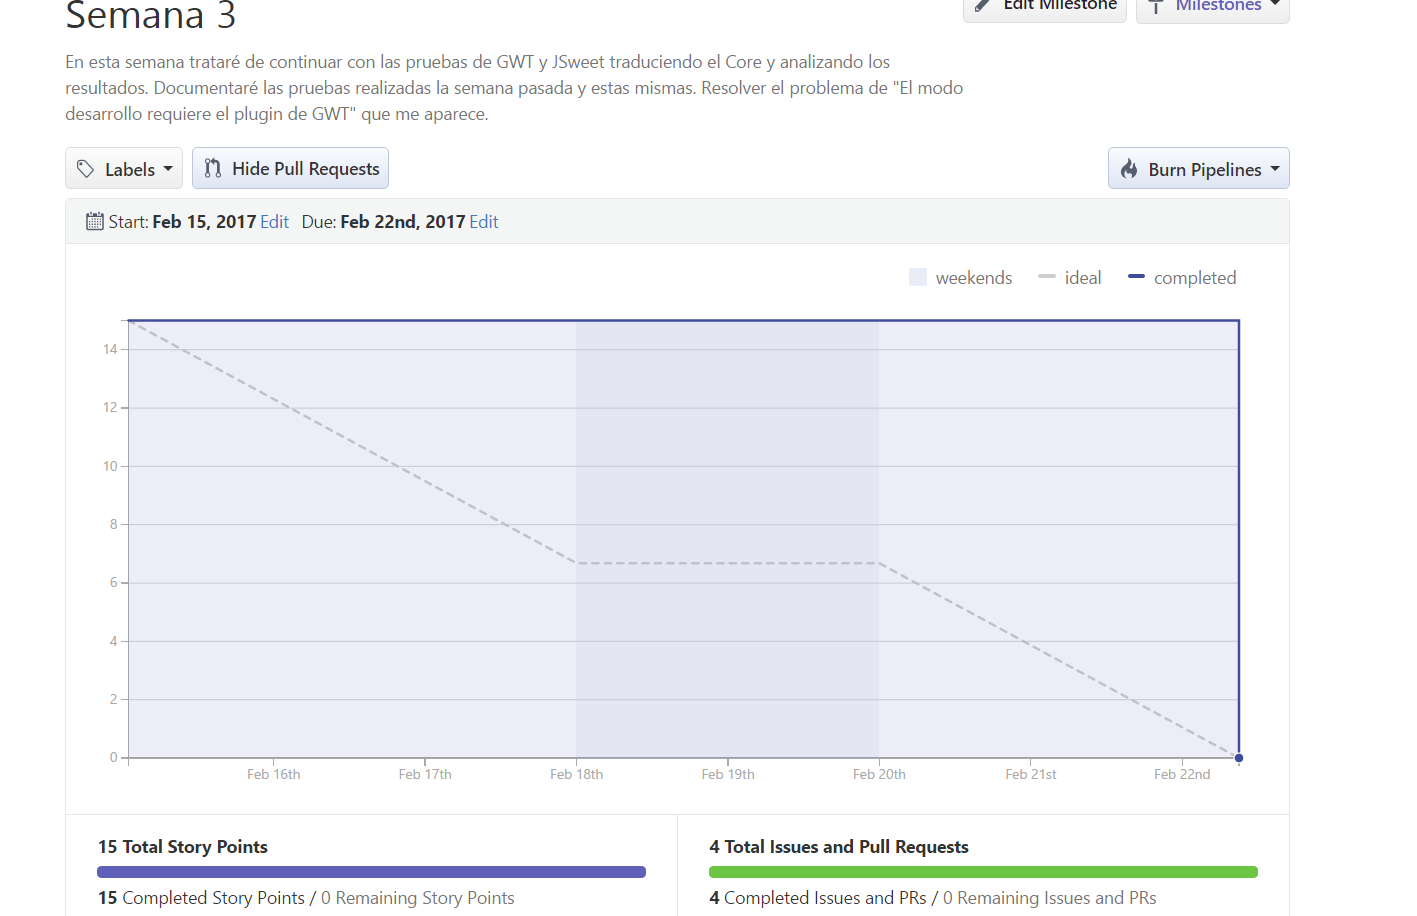
\includegraphics[width=0.99\textwidth]{Semana3}
\caption{Burndown del sprint 2}
\label{fig:A.1}
\end{figure}

También en esta semana descubrimos una nueva herramienta relacionada con el tema, que se llama Vaadin y que nos puede servir, por lo menos para hacer una comparativa más completa de las herramientas de traducción. 

La parte más importante de esta semana es la prueba de traducción del \emph{core} de Thoth, que aunque no sale como esperamos, ha resultado útil para conocer con mayor profundidad tanto la aplicación como la herramienta.

Por lo tanto como tareas para este \emph{sprint}:

\begin{itemize}
\item Solucionar el error surgido con GWT.
\item Realizar pruebas de traducción con el \emph{core} de Thoth.
\item Incluir la nueva herramienta en la comparativa.
\end{itemize}

Muy a mi pesar, en el \emph{milestone} de esta semana, aunque he pasado cada tarea al estado de realizada o <<done>> no las he cerrado hasta darnos cuenta al final del \emph{sprint}, es por ello que el \emph{burndown} queda de esta manera.


\subsection{Sprint 3 (22/2/2017 - 1/3/2017)}

Ya en la cuarta semana se hace un intento más completo para traducir la aplicación. Como pudimos comprobar en la semana pasada, GWT no traducía las librerías de la parte visual de Thoth. Es por ello que decidimos hacer un ejemplo de forma manual que consiste en programar parte de la vista que esta asociada a las partes más relevantes del núcleo.

Por ejemplo, nos centramos en hacer una prueba con la gramática, que está dentro del núcleo, creando una pantalla con un <<text label>> para comprobar si funcionaba la traducción de esa parte del núcleo. De esta forma podríamos ver como hacía la traducción de todo el núcleo, ya que las otras partes de las que se compone son similares en el uso de librerías y bibliotecas.

Quedan así asignadas las tareas para del \emph{sprint} número tres:

\begin{itemize}
\item Transformar la Gramática del núcleo de Thoth.
\item Transformar el Autómata del núcleo.
\item Transformar la simulación del núcleo de Thoth.
\item Documentar toda esta parte.
\end{itemize}

Al final solo se pudo llevar a cabo la tareas de la Gramática y la documentación porque no se pudo avanzar a las otras como muestra la imagen \ref{fig:A.2}.

\begin{figure}[h]
\centering
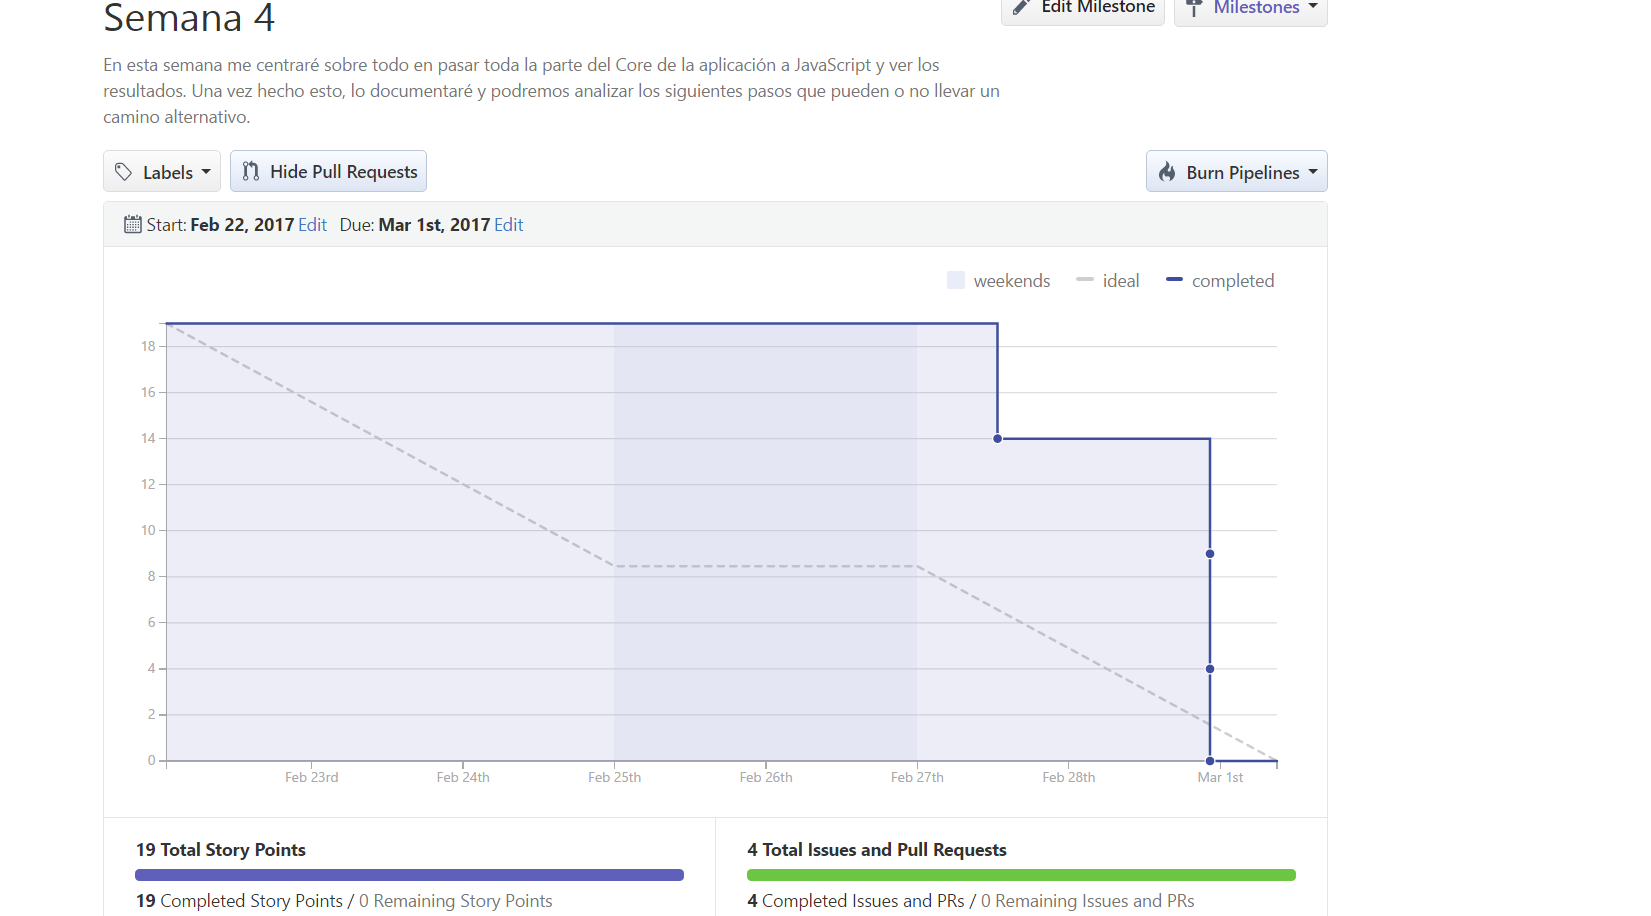
\includegraphics[width=0.99\textwidth]{Semana4}
\caption{Burndown del sprint 3}
\label{fig:A.2}
\end{figure}

 Nuestra idea era probar a tratar de traducir todo, núcleo incluido, ejecutando esas partes en el cliente de GWT  pero vimos que esto no es posible. Intentamos hacerlo de varias formas eliminando partes no esenciales de la aplicación para reducir errores de compilación hasta darnos por vencidos y ver que esa no era la solución.

\subsection{Sprint 4 (1/3/2017 - 8/3/2017)}
Hemos intentado pasar la aplicación en la parte del servidor y probar por nuestra cuenta. Sólo hemos metido el núcleo en el paquete servidor para ver que surgía. Como vimos que no había una comunicación entre el cliente y el servidor hicimos varios intentos, probando con el paquete de \emph{shared} o compartido, pero GWT también traduce ese paquete a JavaScript por lo que seguía dando los mismo errores que en el cliente.

Por lo tanto en este \emph{sprint} tenemos esta tareas:

\begin{itemize}
\item Solucionar un error en la traducción.
\item Realizar pruebas cliente-servidor con el núcleo de la aplicación.
\item Cambios y mejoras en la documentación.
\end{itemize}

Una vez nos dimos cuenta de que el fallo de tratar de hacer la aplicación en la parte del servidor era que GWT no reconocía algunas de las librerías claves, tanto en la parte visual como en el núcleo de la aplicación, decidimos buscar otros caminos alternativos. 


\begin{figure}[h]
\centering
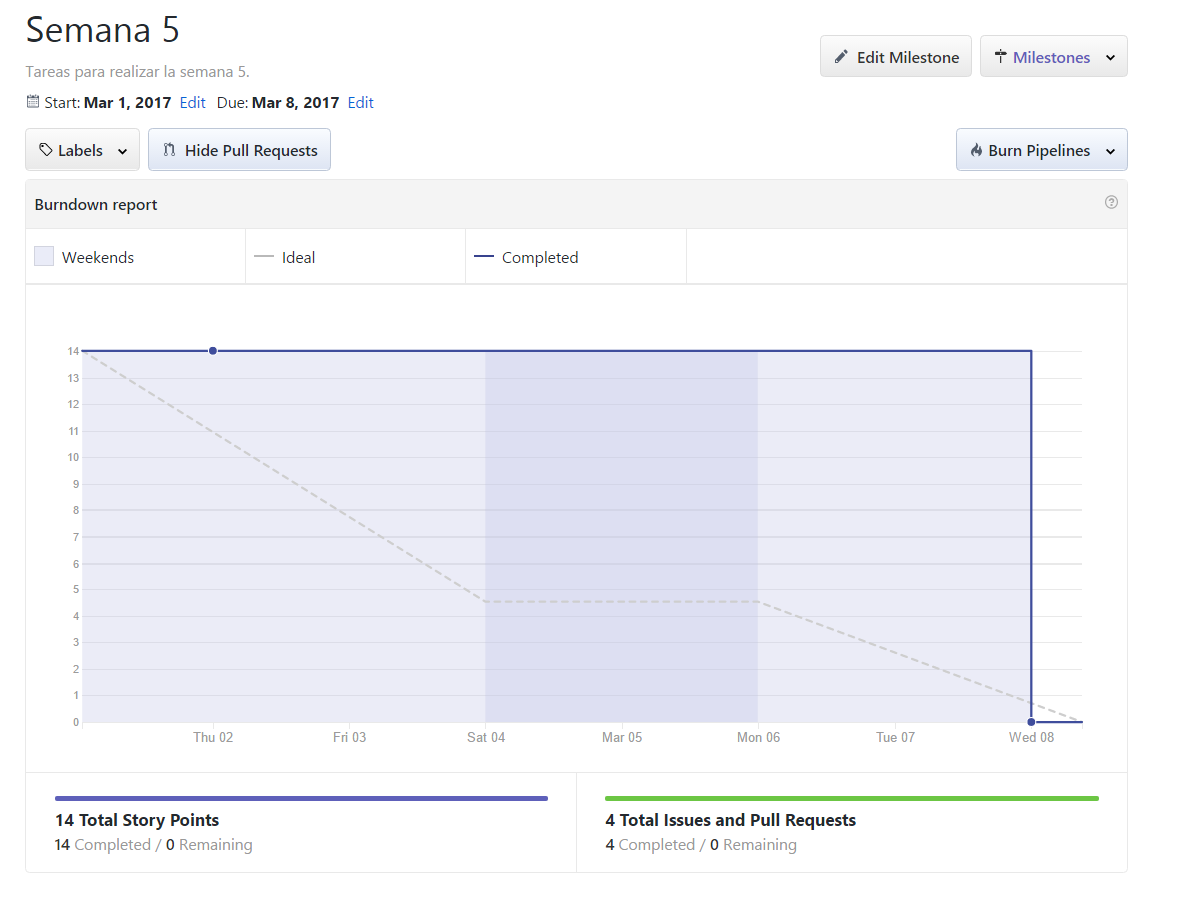
\includegraphics[width=0.99\textwidth]{Semana5}
\caption{Burndown del sprint 4}
\label{fig:A.3}
\end{figure}

El funcionamiento de GWT consiste en traducir a <<JavaScript>> la parte del cliente y la compartida. En consecuencia decidimos hacer pruebas en las que las partes mas fundamentales del núcleo se encontrasen en el lado del servidor. De esta forma cuando el cliente necesitase hacer algún uso de métodos con librerías no reconocidas por GWT, simplemente llamase al servidor ya que este podría soportar dichos métodos. 

En los primeros intentos nos dimos cuenta de que estas llamadas no se podían hacer de una forma simple, ya que la comunicación entre cliente y servidor no funcionaba y no obteníamos los resultados que esperábamos. Aún así seguimos haciendo pruebas para asegurarnos, metiendo dentro del paquete <<compartido>> las partes del núcleo mas cercanas a lo que nosotros consideramos la vista. El problema seguía siendo esa comunicación. Interpretaba como del lado del cliente lo que nosotros queríamos que formara parte del servidor, dando errores debido a que GWT no trabaja con esas librerías.

\subsection{Sprint 5 (8/3/2017 - 15/3/2017)}

Principalmente, en este quinto \emph{sprint}, se llevan a cabo las pruebas para entender y poder evaluar la comunicación cliente-servidor, por medio de unos ejemplos. Además de eso, planteamos la idea de realizar un \emph{login} y validación de usuarios, pero solo como idea, ya que no es prioritario al cien por cien importancia.

\begin{figure}[h]
\centering
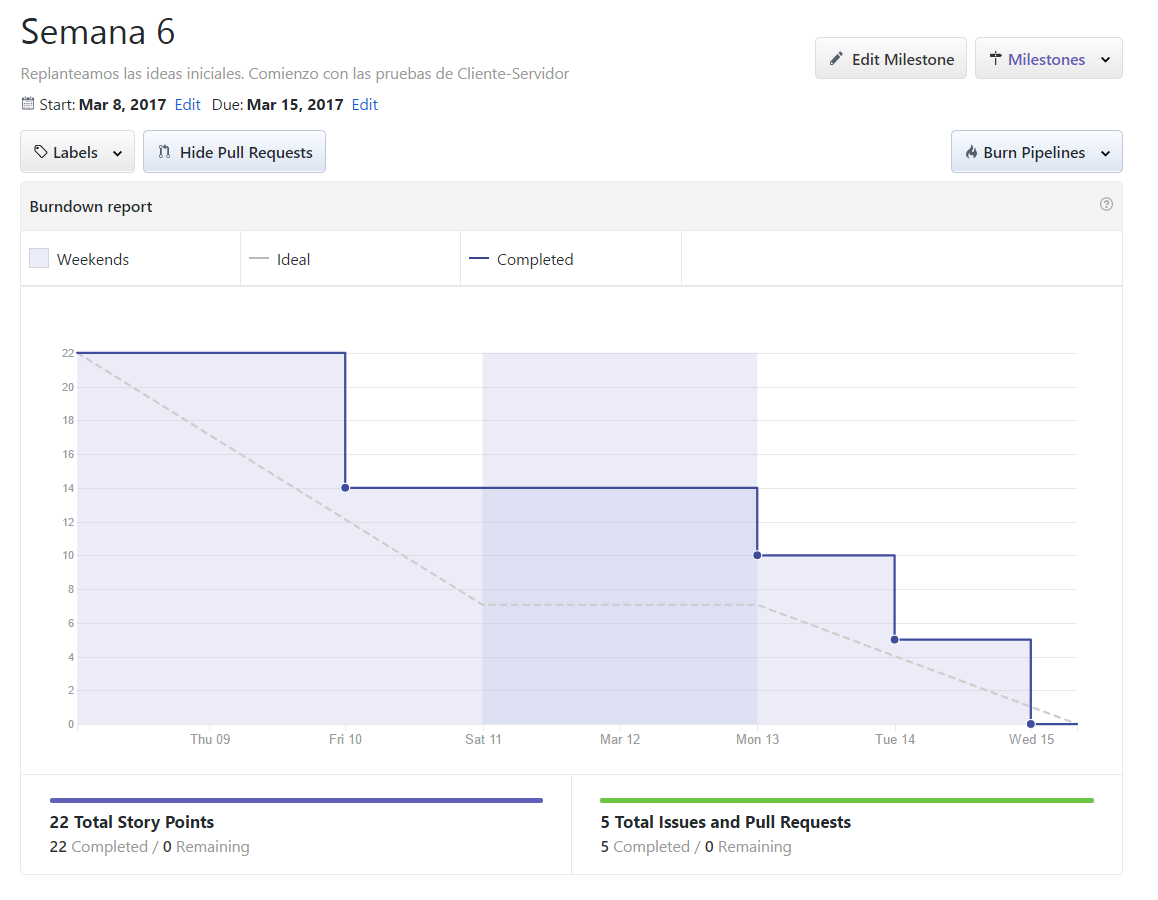
\includegraphics[width=0.99\textwidth]{Semana6}
\caption{Burndown del sprint 5}
\label{fig:A.4}
\end{figure}


Así que en este sprint tenemos esta tareas:

\begin{itemize}
\item Ejemplo cliente-servidor con GWT.
\item Login y validación en GWT.
\end{itemize}

Como se puede ver en el \emph{burdown chart} del \emph{sprint} 5  en la figura \ref{fig:A.4}, se trabajó de forma continuada en esta semana.
La comunicación entre el cliente y el servidor se lleva a cabo mediante la comunicación RPC (\emph{Remote Procedure Call}). Es por ello que se hace necesario entender y practicar el funcionamiento de esta práctica. Los ejemplos realizados han sido dos: el primero es un ejemplo o tutorial ofrecido por la página oficial de GWT, que consiste en hacer un visor del stock que cambia de forma aleatoria sus valores. Y el segundo ejemplo consistió en hacer un pequeño ejemplo de llamada de funciones con más clases que en el anterior.


\subsection{Sprint 6 (15/3/2017 - 22/3/2017)}

En esta semana nos metemos ya en serio con la aplicación propiamente dicha. Lo primero que hacemos es conseguir que la comunicación entre en núcleo (ya hecho) y su uso sea fluido. Para ello lo que hacemos es incluir algunas partes en el cliente y otras en el servidor. En el cliente sólo podemos incluir las clases más simples, más primitivas de la aplicación porque su contenido es entendido por GWT y puede hacer la traducción a JavaScript sin problemas de librerías.

\begin{figure}[h]
\centering
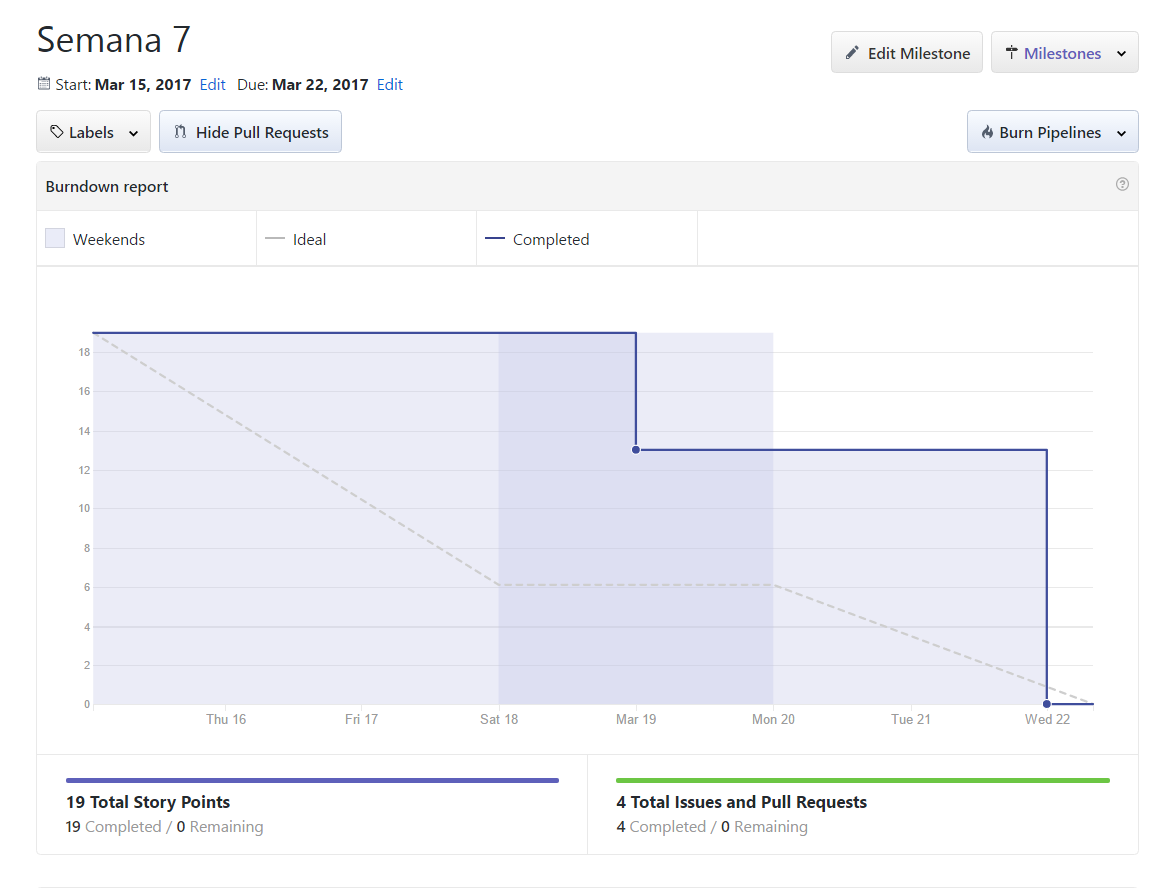
\includegraphics[width=0.99\textwidth]{Semana7}
\caption{Burndown del sprint 6}
\label{fig:A.5}
\end{figure}

Por lo tanto las tareas son básicamente dos:

\begin{itemize}
\item Llevar a cabo el primer prototipo o sección de la aplicación.
\item Documentar y corregir errores anteriores en la documentación.
\end{itemize}

La realización del prototipo nos lleva tiempo ya que se necesita comprender muy bien el funcionamiento interno de Thoth y así poder definir un diseño del software adecuado según ese funcionamiento. Una vez hecho eso parece simplificarse los problemas que al principio se tenían. Puede verse el \emph{burdown chart} de este \emph{sprint} en la figura\ref{fig:A.5}.

\subsection{Sprint 7 (22/3/2017 - 29/3/2017)}

Parece ser que en esta octava semana ya podemos empezar a trabajar más en la programación del diseño e implementar funcionalidades. Lo primero que tenemos que hacer es que esa comunicación entre métodos de resultados <<más>> visibles e integrarlos en una <<GUI>> denominada en español como interfaz gráfica de usuario. Para más detalles sobre la semana, ver la figura\ref{fig:A.6}

Así es que definimos como tareas las siguientes:

\begin{itemize}
\item Reestructurar la aplicación y limpiar el código.
\item Mejorar la GUI con Vaadin, ya que la anterior es muy básica.
\item Implementar el algoritmo "Eliminar símbolos no terminales"
\end{itemize}

\begin{figure}[h]
\centering
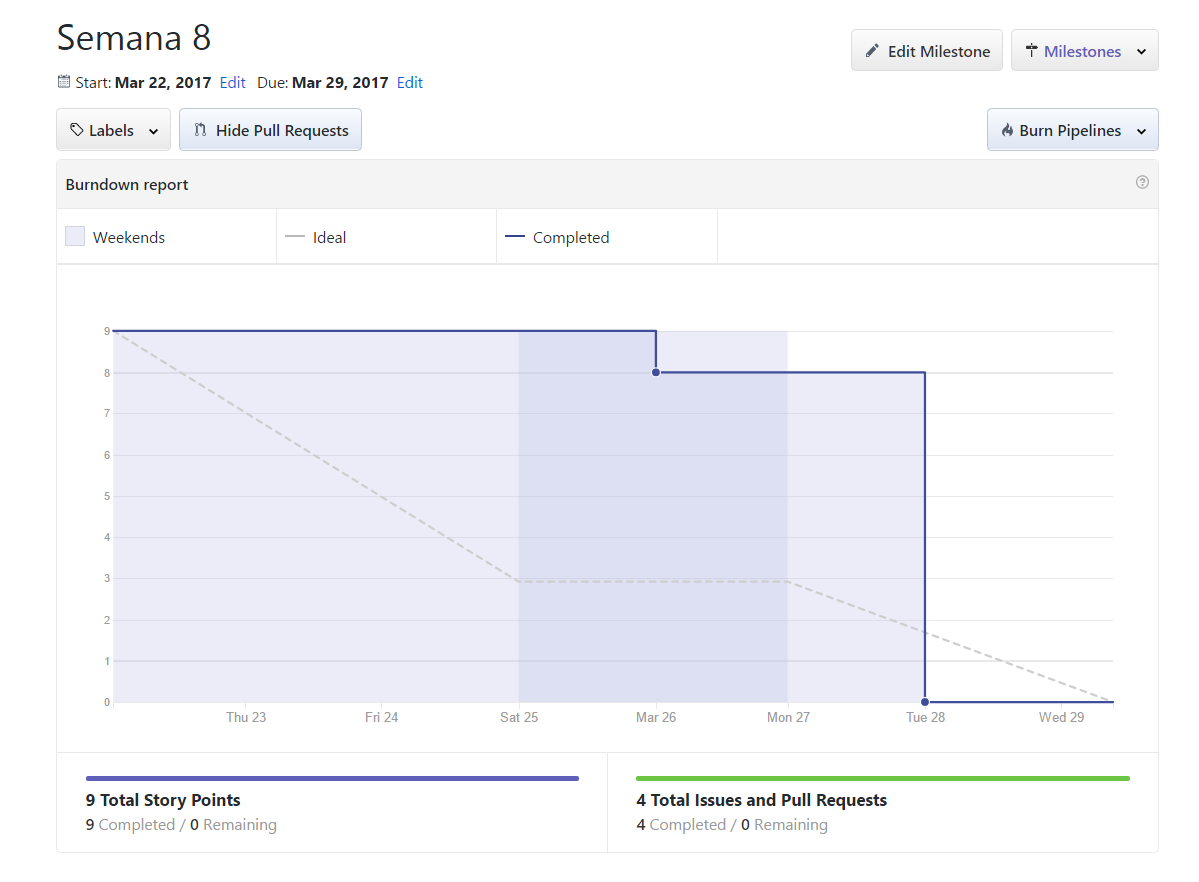
\includegraphics[width=0.99\textwidth]{Semana8}
\caption{Burndown del sprint 7}
\label{fig:A.6}
\end{figure}

Primeramente hay que organizar el código haciéndolo más legible y limpiarlo de comentarios, y pruebas para ver su funcionamiento. Queremos que los resultados queden de una forma similar al Thoth original, para conservar su esencia, usabilidad, y buen diseño. Para ello hacemos uso de Vaadin, una herramienta que se puede utilizar como un \emph{plugin} en eclipse y que se integra perfectamente con GWT.

\subsection{Sprint 8 (29/3/2017 - 5/4/2017)}

Al principio de este octavo \emph{sprint} o 9 semana, estuve pendiente de la respuesta por parte de Vaadin sobre si me podía conceder o no una licencia gratuita, así que me centré en incluir el algoritmo de eliminación de símbolos no terminales, mejorando lo que tenía hasta el momento, que era solo una pequeña interfaz con una funcionalidad que no era la exacta. Por ello me centré en corregirla. Así lo hicimos.

\begin{figure}[h]
\centering
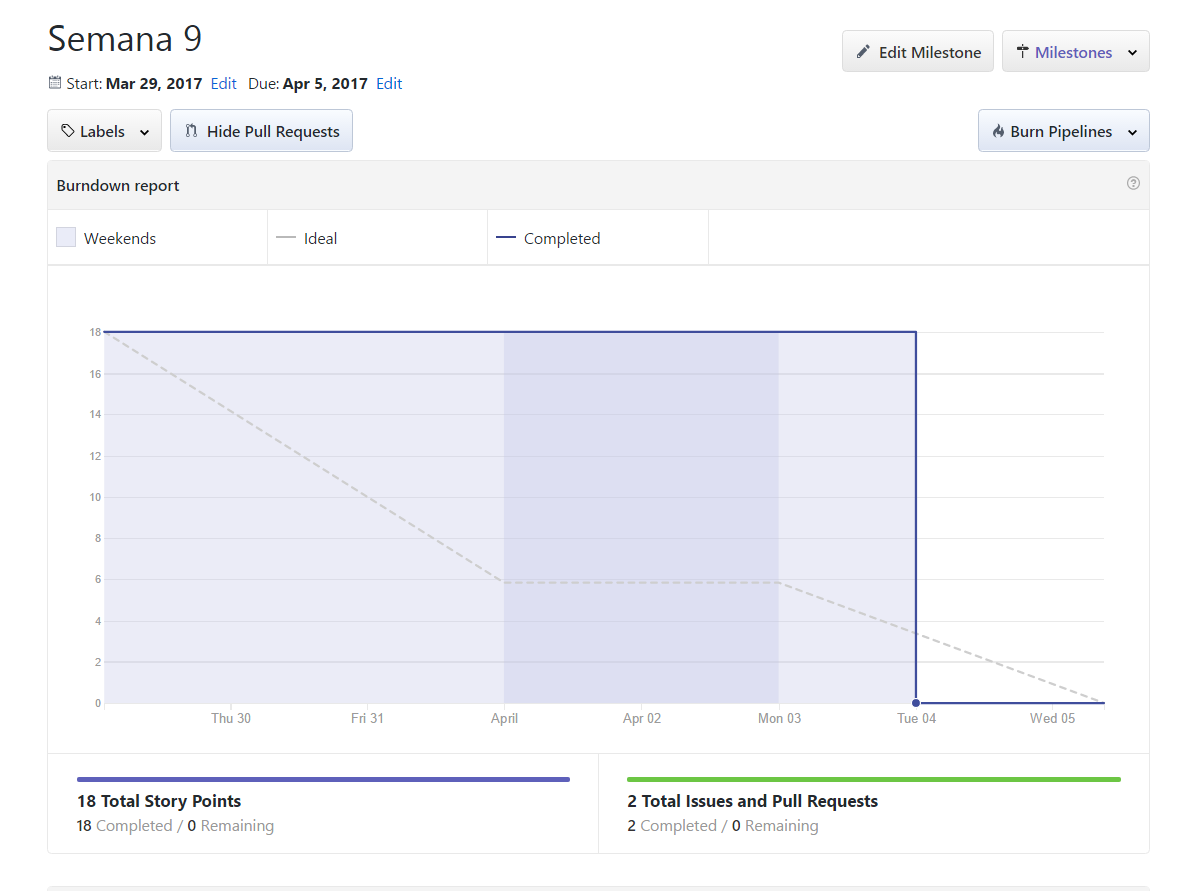
\includegraphics[width=0.99\textwidth]{Semana9}
\caption{Burndown del sprint 8}
\label{fig:A.7}
\end{figure}

Posteriormente llegó la respuesta de Vaadin explicando que no me podía conceder la licencia y que buscase otras opciones dentro de las que ellos mismos me ofrecían. Al principió lo intenté pero resulto que no supe como hacerlo. Lograba hacer un proyecto de Vaadin pero no conseguía incluirlo en el mío propio de GWT.

Así que comencé a hacer la interfaz por mi mismo, con las posibilidades de GWT. Puede verse en el \emph{burdown chart }de la ilustración \ref{fig:A.7} como la carga de trabajo se concentra sobre todo en el final.

Las tareas para esa semana fueron: 

\begin{itemize}
\item La inclusión del algoritmo de Eliminación de símbolos no terminales, de una forma mejorada.
\item Recabar información sobre internacionalización en GWT.
\end{itemize}

Logramos hacer que funcionase el algoritmo como queríamos y estuvimos mejorando el diseño y la funcionalidad de la interfaz de dicho algoritmo.

\subsection{Sprint 9 (05/4/2017 - 19/4/2017)}

Es el \emph{sprint} más largo hasta la fecha ya que incluye dos semanas de trabajo por coincidir con las vacaciones de Semana Santa. Engloba fundamentalmente el hacer los demás algoritmos, con sus respectivas vistas. El \emph{burdown chart} del \emph{sprint} 9 se ilustra en la figura \ref{fig:A.8}.

\begin{itemize}
\item Implementar los algoritmos restantes.
\item Mejorar el código, haciéndolo más comprensible y organizar la parte visual.
\item Hacer la documentación sobre la parte del diseño y sobre las herramientas que tiene la UBU relacionadas con este proyecto.
\end{itemize}

\begin{figure}[h]
\centering
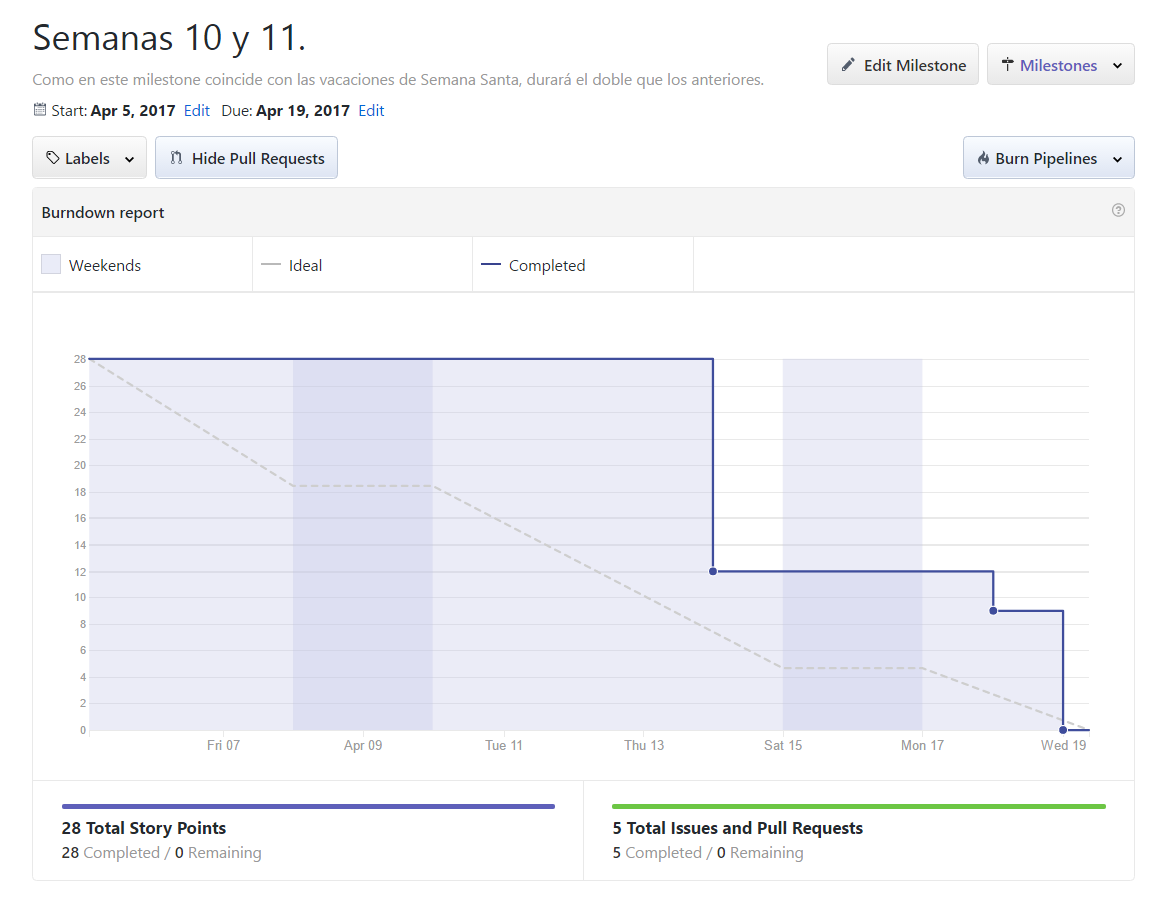
\includegraphics[width=0.99\textwidth]{Semana10-11}
\caption{Burndown del sprint 9}
\label{fig:A.8}
\end{figure}

En estas dos semanas no pude realizar todos los algoritmos como en un principio pretendía porque la parte visual se alejaba de lo que tenía hecho hasta el momento, es decir, necesitaba hacer nuevas vistas que llevaban más tiempo del pensado y no me dio tiempo, pero si que incluí la mayor parte de ellos. Estuvimos estudiando como aplicar el resaltado de las producciones. En el Thoth original utilizaba una librería, java swing, que ya comprobamos anteriormente que no podía ser incluida en GWT en este proyecto así que buscamos otras alternativas como hacer un resaltado a mano con HTML. De momento lo dejamos ahí.

\subsection{Sprint 10 (19/4/2017 - 26/4/2017)}

Una vez pasadas las vacaciones de Semana Santa, el proyecto tiene una forma más madura y podemos ir haciendo añadidos más funcionales a la aplicación. Es por ello que decidimos empezar con la internacionalización, viendo como funcionaba para poder entenderla y una vez entendida incluirla en el proyecto. Además de esto, después de comprobar en la semana pasada que el resaltado lo podíamos hacer con HTML nos dedicamos de lleno a ello. La verdad es que nos llevó muchos quebraderos de cabeza. El porqué no era otra cosa que teníamos que tener en cuenta todo el funcionamiento interno, <<destripar>> que contenía cada variable, como funcionaban cada método de GWT etc. Todo este trabajo nos llevo mucho tiempo, ya que estuvimos todo el \emph{sprint} a base de prueba y error con los diferentes algoritmos hasta que funcionó en todos de la forma que deseamos. En el \emph{burdown chart} \ref{fig:A.9} se puede apreciar como no es hasta el final del \emph{sprint} cuando se cierran los \emph{issues}.

\begin{figure}[h]
\centering
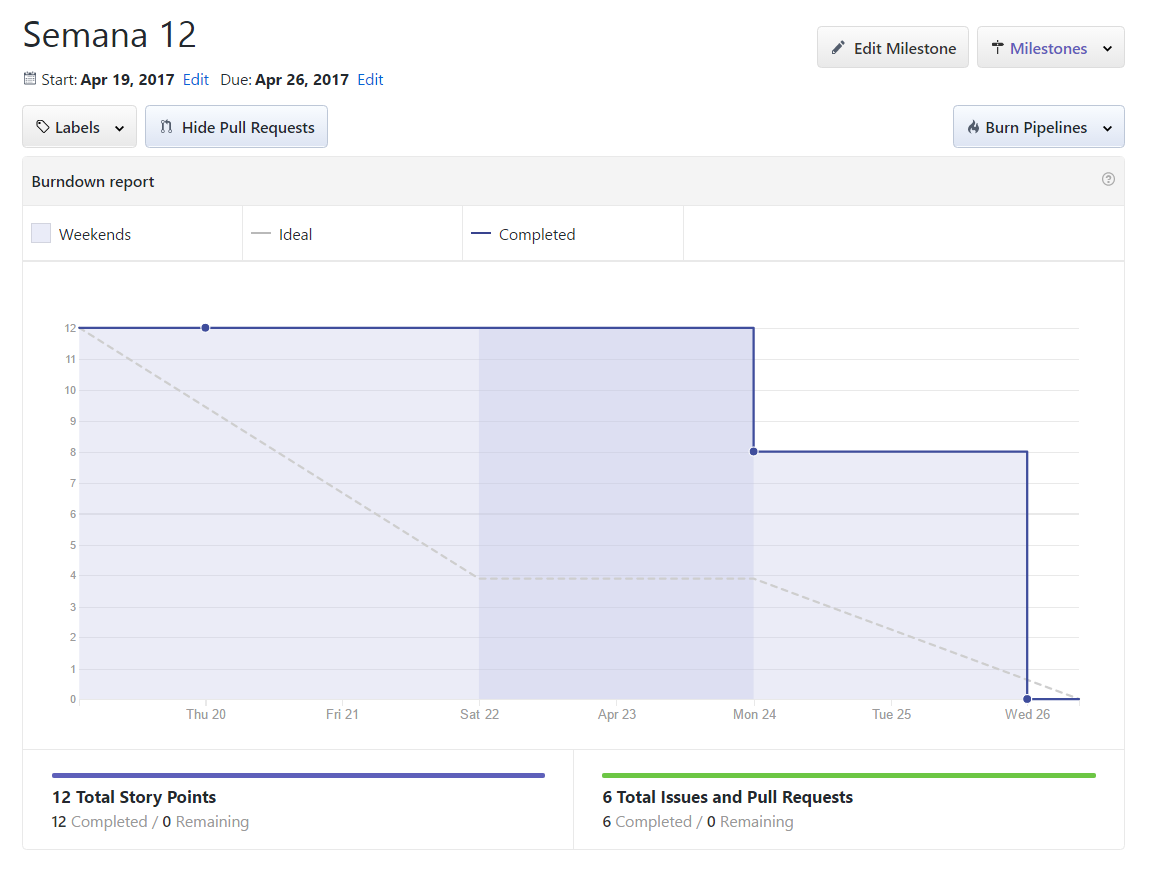
\includegraphics[width=0.99\textwidth]{Semana12}
\caption{Burndown del sprint 10}
\label{fig:A.9}
\end{figure}

Estas fueron las tareas correspondientes a esta semana.

\begin{itemize}
\item Aplicar internacionalización.
\item Cambiar la visualización de los paneles.
\item Resaltado de producciones en los algoritmos con HTML.
\item Incluir los demás algoritmos.
\item Incluir pestañas y elementos de Vaadin.
\end{itemize}

La parte visual, es decir, la inclusión de pestañas en realidad no lo llegamos a aplicar bien, de la forma deseada y se trató en el siguiente \emph{sprint}. Además los elementos de Vaadin no se pudieron incluir ya que la única forma de añadirlos a un proyecto GWT son con licencias de pago. La visualización de los paneles simplemente fue una recolocación para que quedase más agradable a la vista.


\subsection{Sprint 11 (26/4/2017 - 03/5/2017)}

En esta semana seguimos acumulando un pequeño <<bug>> en el resaltado de las producciones, y es que la interpretación de las comillas dobles <<``''>> no las interpretaba como nosotros queríamos y por ello no hacía un buen borrado del resaltado, manteniéndose en cada paso. La solución fue simplemente sustituirlas por las comillas dobles de java <</``>>. Pero las dos grandes tareas de esta semana consistieron en aplicar el algoritmos \emph{FirstFollow} y un \emph{TabLayoutPanel} para hacer un panel con pestañas como los que se ven en los navegadores web.

Las tareas quedaron así.

\begin{itemize}
\item Solucionar \emph{bug} en el resaltado.
\item Implementar algoritmo \emph{FirstFollow}.
\item Incluir \emph{TabLayoutPanel} para hacer diferentes pestañas.
\end{itemize}

El algoritmo \emph{FirstFollow} fue fácil hasta el momento de mostrar los resultados en las tablas. Resulta que al tratar de imprimir los resultados de tipo \emph{Object} pasándolos como un \emph{string} no los reconocía bien. Este tipo de errores no son fáciles de detectar en GWT, ya que la forma para verlos claramente es imprimiendo los valores por pantalla y tratando de analizarlos, en que formato están etc. Al final descubrimos que el problema era al tratar de pasara al formato string valores que GWT interpretaba como \emph{undefined} y que no eran más que valores en blanco, espacios en blanco dentro de la tabla. Se pueden ver mas detalles en la figura \ref{fig:A.10}.

\begin{figure}[h]
\centering
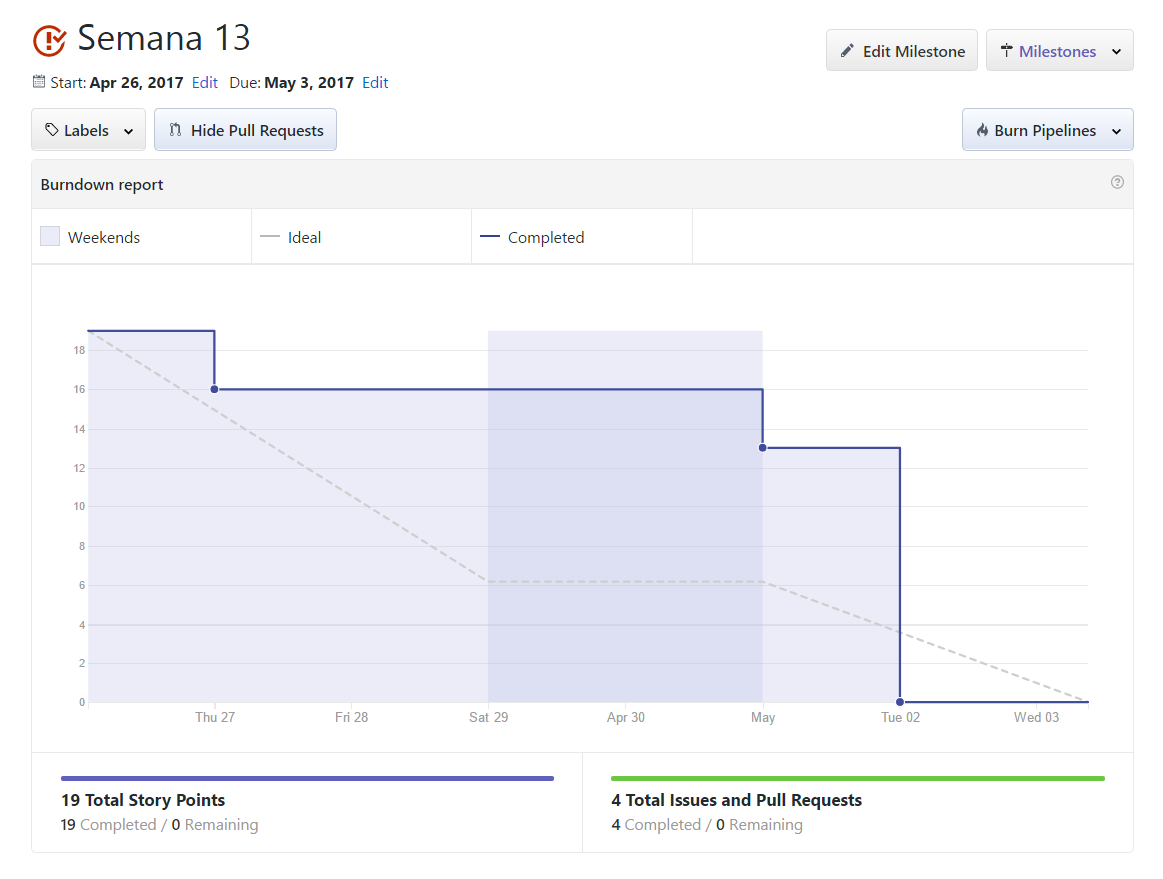
\includegraphics[width=0.99\textwidth]{Semana13}
\caption{Burndown del sprint 11}
\label{fig:A.10}
\end{figure}

El otro gran quebradero de cabeza fue el tratar de incluir pestañas en la aplicación. No es nada fácil añadir una pestaña con una nueva vista sin que esta remplace otra, se superponga o cualquier otra cosa. A día de hoy no sabemos bien el porqué de esto al cien por cien. Lo que si es cierto es que no es completamente necesaria y se puede hacer un reemplazamiento de otras vistas.

\subsection{Sprint 12 (03/5/2017 - 10/5/2017)}

Entrado en el mes de mayo, la recta final del proyecto, y con una aplicación base ya consolidada, por denominarlo así, nos dedicamos sobre todo ha hacer mejoras en cuanto a temas visuales y funcionales. Además de esto el objetivo en este mes es hacer un registro e inicio de sesión de los usuarios para así tener un control detallado del uso.
Con todo esto por un lado, también era hora de dedicarle un porcentaje de tiempo mayor a documentar el proyecto. Véase la ilustración \ref{fig:A.11}.

\begin{figure}[h]
\centering
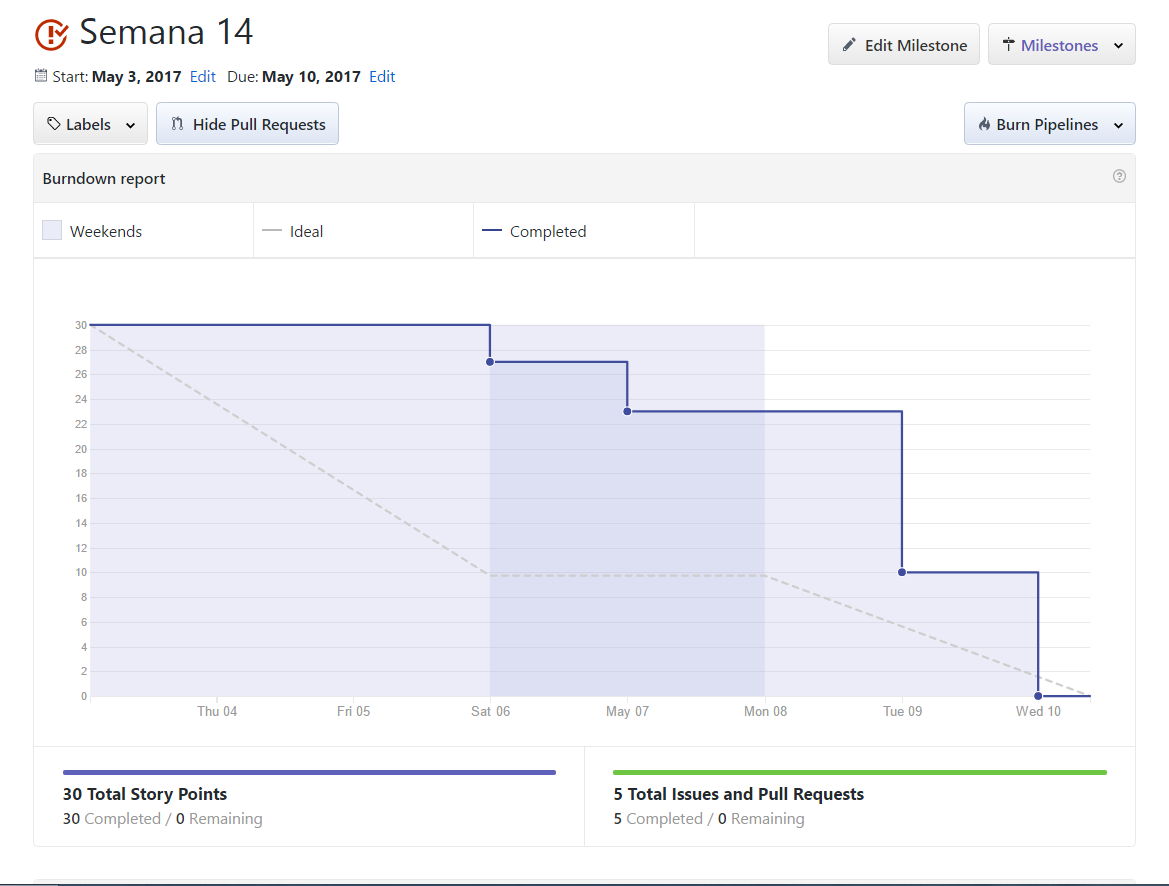
\includegraphics[width=0.99\textwidth]{Semana14}
\caption{Burndown del sprint 12}
\label{fig:A.11}
\end{figure}

Para esta semana determinamos que las tareas quedaría de esta manera:

\begin{itemize}
\item Comenzar a estudiar y probar el inicio de sesión.
\item Actualizar la documentación.
\item Mejoras en la interfaz (botones, colores y formas).
\item Añadir un control de errores más elaborado y hacer la aplicación más robusta.
\item Cambiar la funcionalidad de los botones en los algoritmos.
\end{itemize}

La tarea de cambiar la funcionalidad de los botones en los algoritmos hace referencia a que regrese o vaya a una vista u otra dependiendo del botón pulsado o de las acciones asociadas a ello.
Las mejoras visuales son hechas a mano, como ya he comentado anteriormente, y es por ello que es un trabajo largo, en el que hay que estar compilando continuamente para ver los efectos resultantes, que no siempre son los esperados.
El inicio de sesión acabó en un ejemplo con varios errores y algo chapucero que sirvió para comprender el funcionamiento por lo que no se mejoró nada en la aplicación.

\subsection{Sprint 13 (10/5/2017 - 17/5/2017)}

Llegados a este punto comenzamos a <<pulir>> lo que tenemos añadiendo estilos con CSS y mejorando pequeños aspectos como es el caso de la vista de los algoritmos. Al resaltar los pasos en un algoritmo, tuvimos la <<necesidad>> de utilizar un \emph{RichTextArea} para poder manejar el código HTML y poder así subrayarlo. Más tarde nos dimos cuenta de que este tipo de área no se puede inhabilitar para que no se editable y esto se trata de un bug de GWT, la función está pero no hace nada. Otros usuarios también se quejaron de ello\footnote{\url{https://code.google.com/archive/p/google-web-toolkit/issues/1488}}. Así que decidimos meterlo todo dentro de un panel como texto normal en HTML, que al fin y al cabo era lo que ya habíamos hecho. El \emph{burdown chart} se ilustra en la figura \ref{fig:A.12}.

Los issues quedaron definidos así:
\begin{itemize}
\item Cambiar las interfaces de las gramáticas.
\item Incluir nuevos estilos.
\item Documentar aspectos como la introducción y los conceptos teóricos.
\item Añadir una nueva clase para hacer la internacionalización.
\item Solucionar un bug que surgió sobre la vista de los algoritmos.
\item Aplicar un pequeño ejemplo de inicio de sesión.
\end{itemize}

\begin{figure}[h]
\centering
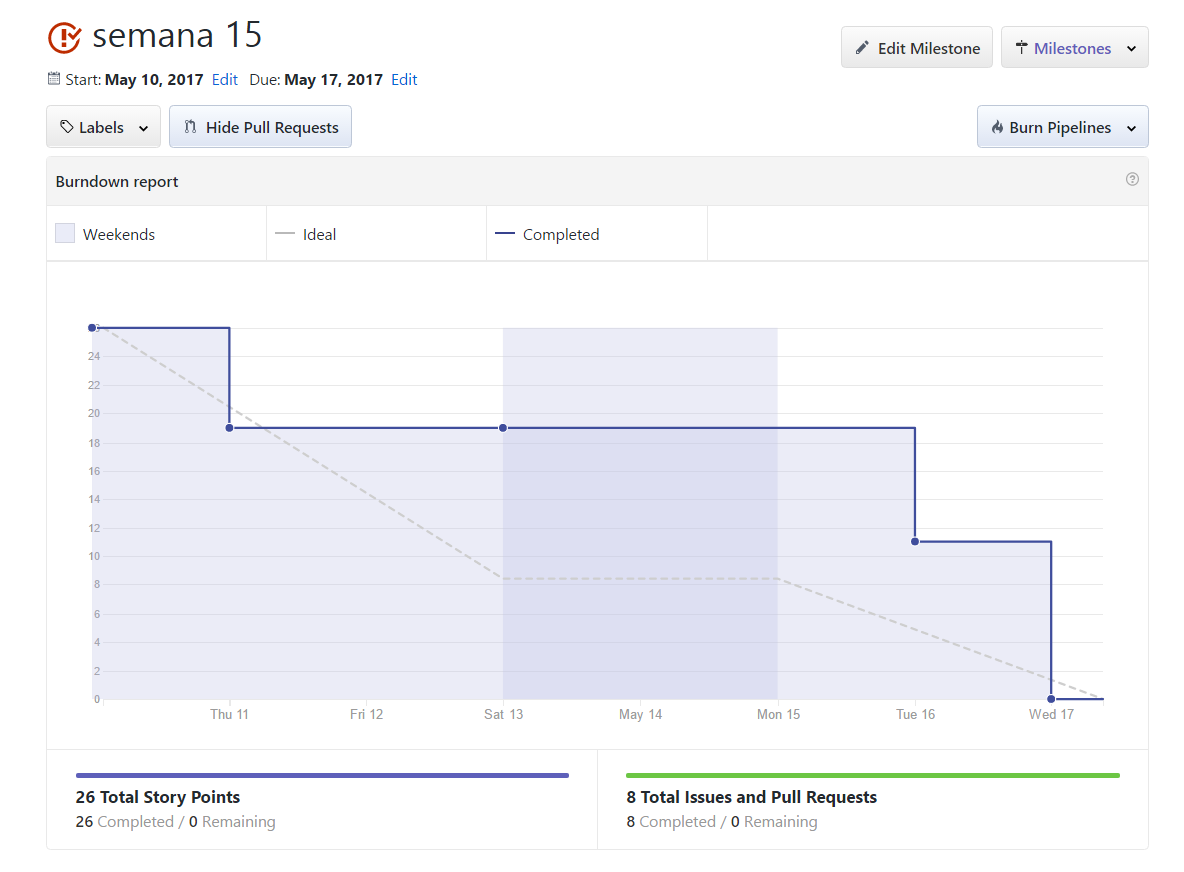
\includegraphics[width=0.99\textwidth]{Semana15}
\caption{Burndown del sprint 13}
\label{fig:A.12}
\end{figure}

Se pudo hacer un ejemplo en un proyecto a parte para hacer un simple inicio de sesión sin base de datos. Para lograr el inicio se hizo por medio de \emph{cookies}. El objetivo siguiente sería poder aplicar esto a nuestro proyecto pero con una pequeña base de datos en la cual se registraban los usuarios y luego hacían inicio de sesión. También añadimos clases para que encapsularan la internacionalización y poder lanzar mensajes de aviso.

\subsection{Sprint 14 (17/5/2017 - 24/5/2017)}

En el \emph{sprint} 14, es decir la decimosexta semana, se centraron los esfuerzos sobre todo en hacer un registro e inicio de sesión de usuarios. La idea inicial era la de guardar información de nombre, apellido, un correo que sirviera de identificador único y una contraseña. Para ello se creó una pequeña base de datos, casi podríamos hablar de repositorio. Una vez registrados esos datos el usuario tendría un perfil creado y podría acceder a la aplicación.

Las tareas se centraron en documentar y hacer el registro y sesión de usuarios:
\begin{itemize}
\item Añadir un \emph{login} o inicio se sesión.
\item Corregir aspectos de la documentación.
\item Incluir alguna mejora en el menú principal.
\end{itemize}

\begin{figure}[h]
\centering
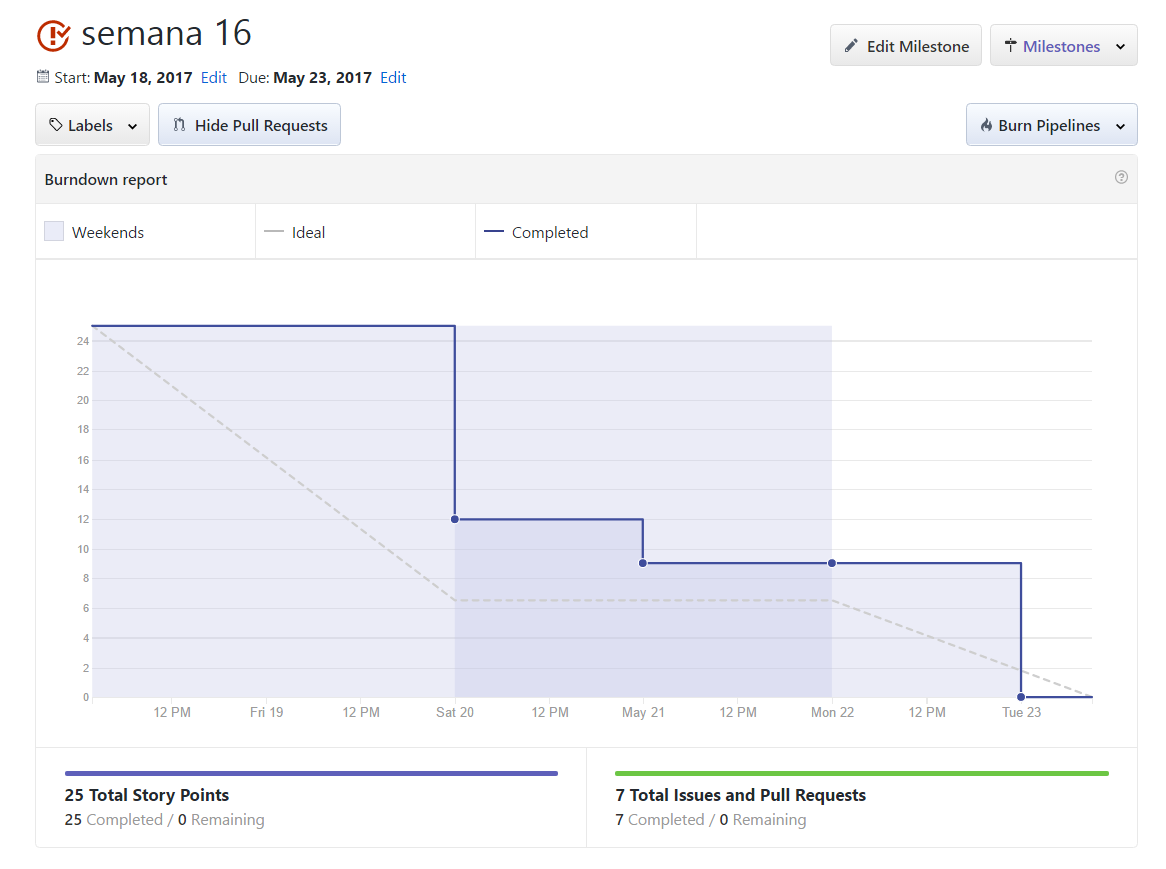
\includegraphics[width=0.99\textwidth]{Semana16}
\caption{Burndown del sprint 14}
\label{fig:A.13}
\end{figure}

Además de esto, surgió un \emph{bug} o pequeño error con los estilos <<css>>. Y es que al crear varios módulos para realizar varias vistas en la aplicación los estilos, que son propios de cada módulo, se solapaban y se mezclaban mostrando en un módulo el estilo del otro y viceversa. El error no tenía mucha complicación y se pudo solucionar sin problema. Puede verse el \emph{burdown} en la ilustración \ref{fig:A.13}.
El registro e inicio de sesión me llevo tiempo, dos \emph{sprints} el hacer lo básico y otros dos <<pulirlo>> ya que los conceptos en cuanto a carga de módulos, y comunicación RPC eran en parte nuevos. Lo demás fue principalmente documentación, mejorarla y continuar con lo anterior.

\subsection{Sprint 15 (24/5/2017 - 31/5/2017)}

Ya en la semana 17, una vez que tenemos la base de datos haciendo el registro de usuarios, nos metemos con la codificación de las contraseñas. Consiste en crear una clave secreta generada por medio de una función con la que ciframos la contraseña para mantener la privacidad de los datos de los usuarios registrados. 

Los \emph{issues} para este sprint son:
\begin{itemize}
\item Cifrado de contraseñas.
\item Registro de más información.
\item Mejorar el aspecto del \emph{login}.
\end{itemize}

El registro de más información consiste en añadir a la base de datos la fecha de registro de un usuario o la última vez que inició sesión en la aplicación. La resolución de los \emph{issues} queda reflejada en la siguiente gráfica ilustrada en la figura \ref{fig:A.14}.

\begin{figure}[h]
\centering
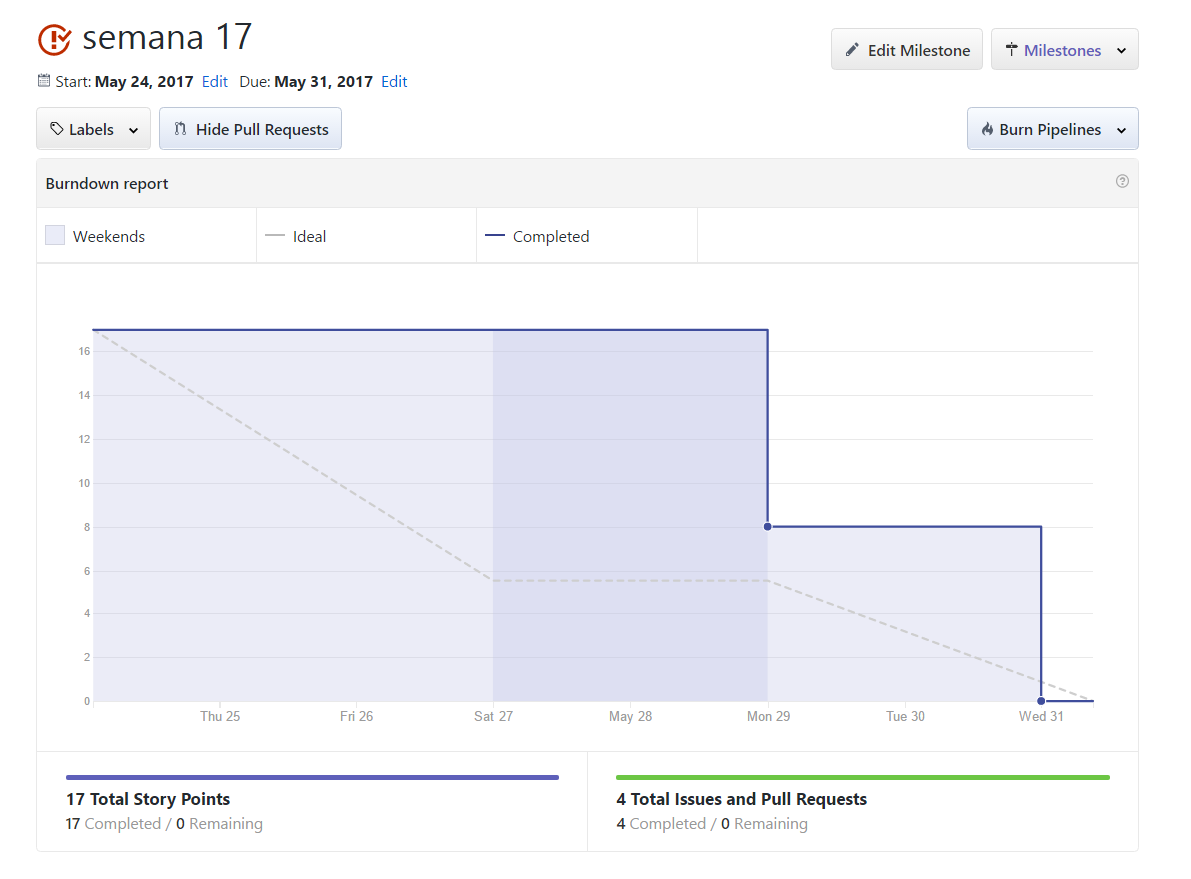
\includegraphics[width=0.99\textwidth]{Semana17}
\caption{Burndown del sprint 15}
\label{fig:A.14}
\end{figure}

Además de esto, añadimos algunos estilos a las vistas de inicio y registro de sesión aunque posteriormente lo volveremos a modificar, hasta estar a gusto con el diseño.

\subsection{Sprint 16 (31/5/2017 - 7/6/2017)}

En el \emph{sprint} número dieciséis tratamos de pulir un poco lo que tenemos. Para ello limpiamos el código refactorizando y dando nombres a las variables con un sentido más específico, comentando un poco el código y eliminando aquello que no nos es útil. Arreglamos algún \emph{bug} que aparece en el renombrado de nodos por ejemplo.


Para esta semana las tareas son las siguientes.
\begin{itemize}
\item Cifrado de contraseñas.
\item Validación de \emph{e-mail}.
\item Añadir tratamiento de errores en el \emph{login}.
\item Refactorizar el código.
\end{itemize}

Seguimos con el cifrado de contraseñas porque decidimos mejorarlo y dejarlo más claro y con más posibilidades, dependiendo de las interacciones y de las variables podemos crear un nivel de cifrado más simple o más complejo. 

A su vez comprobamos que la dirección de correo introducida cumpla con la <<plantilla>> de una dirección real. Consiste en hacer una comprobación por medio de HTML y una función en Java bastante simple. El \emph{burdown} queda de esta manera \ref{fig:A.15}.

\begin{figure}[h]
\centering
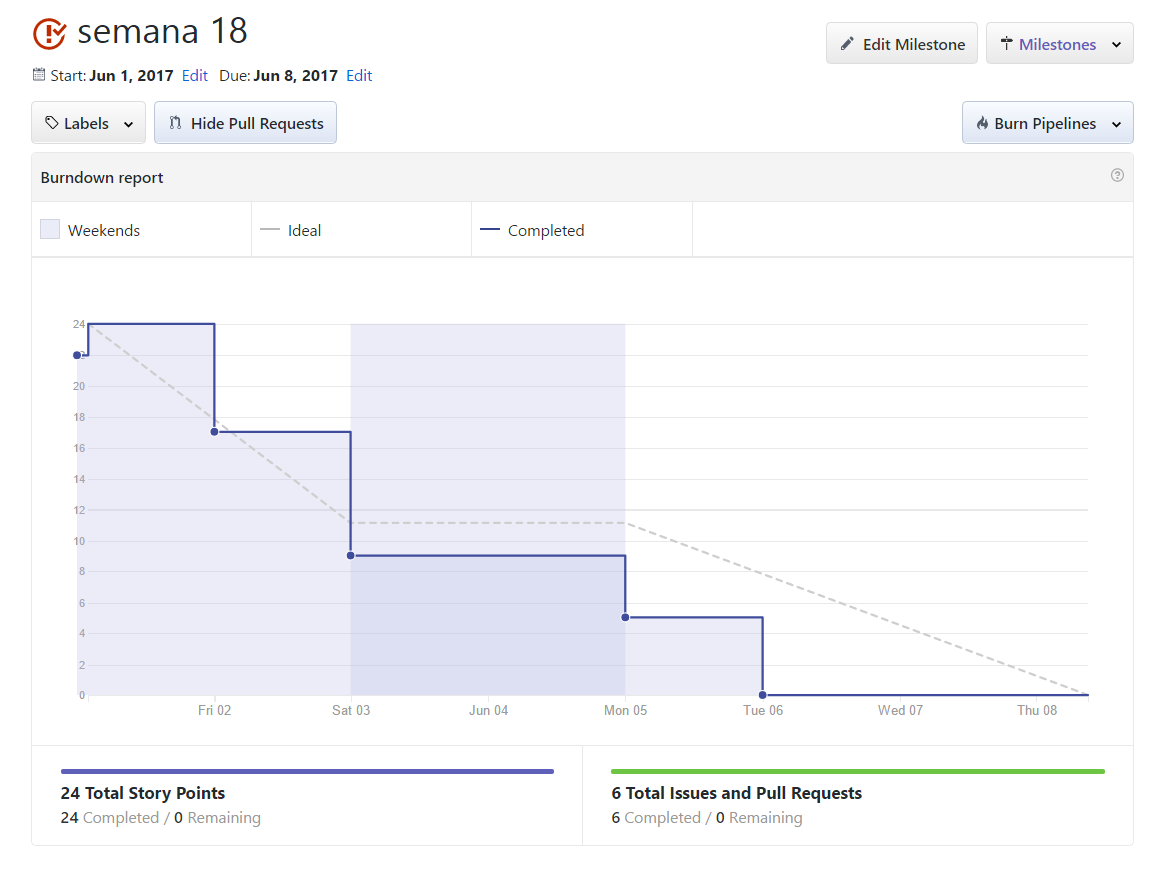
\includegraphics[width=0.99\textwidth]{Semana18}
\caption{Burndown del sprint 16}
\label{fig:A.15}
\end{figure}

Además de esto añadimos imágenes de fondo, el escudo de la universidad de Burgos en el inicio de sesión y registro de usuarios. Esta semana tiene un poco menos de carga de trabajo porque coincide con fechas de exámenes.

\subsection{Sprint 17 (7/6/2017 - 14/6/2017)}

En esta semana, ya centrados en la documentación, pretendemos hacer una mejora importante en el proyecto que consiste en incluir un control de sesiones. Hasta ahora el usuario podía registrarse y hacer \emph{login}, pero aún así podía acceder a la edición de una gramática.

Como hicimos en el \emph{sprint} numero 12 en un prototipo, trataremos de aplicar esto a nuestro proyecto.

Para esta semana las tareas son las siguientes.
\begin{itemize}
\item Documentación de conceptos teóricos.
\item Documentación de del seguimiento del proyecto.
\item Cambios en la interfaz de los algoritmos.
\item Control de sesiones.
\end{itemize}

\begin{figure}[h]
\centering
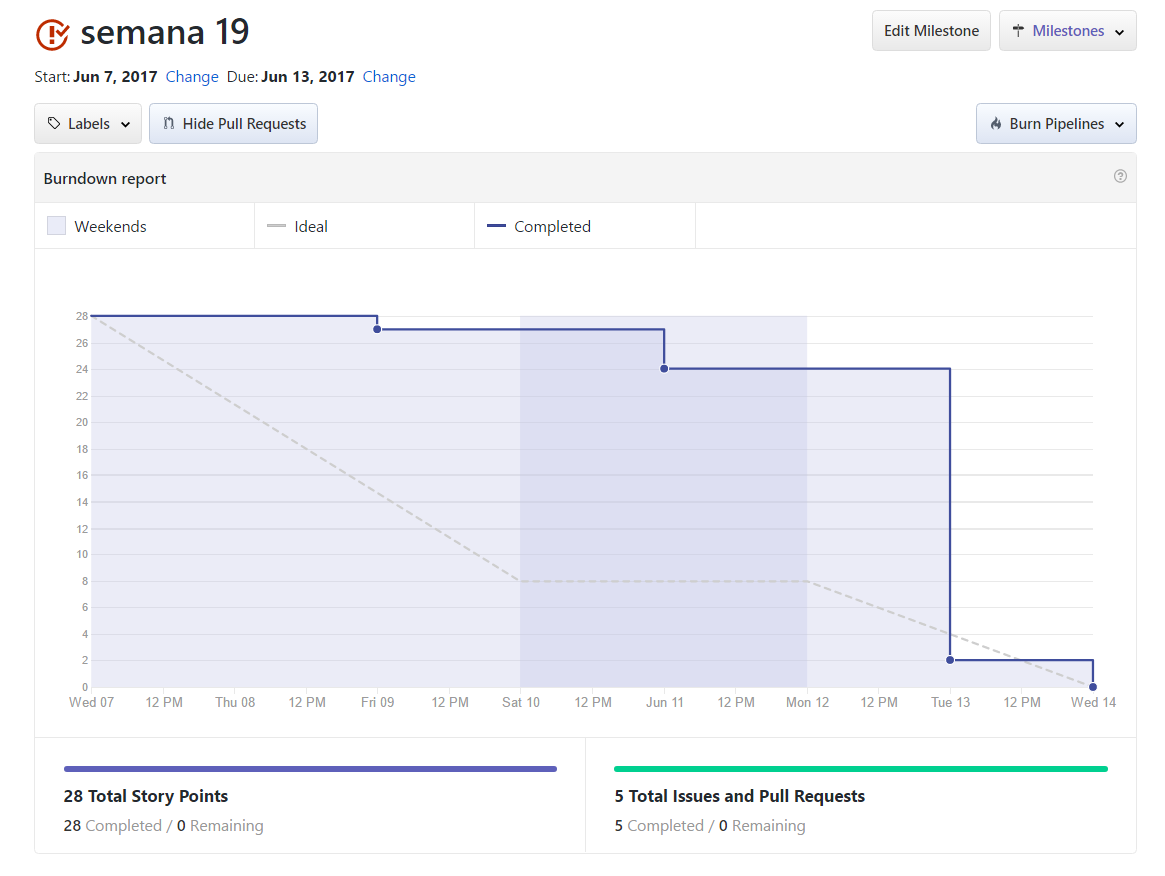
\includegraphics[width=0.99\textwidth]{Semana19}
\caption{Burndown del sprint 17}
\label{fig:A.16}
\end{figure}

Nos lleva trabajo hacer el control de sesiones porque hay que probar cada acción volviendo a compilar el proyecto una y otra vez. Se pueden ver la gráfica de esta semana \ref{fig:A.16}.

\subsection{Sprint 18 (14/6/2017 - 21/6/2017)}

Como ya hemos hecho en las anteriores semanas, documentaremos la memoria sobre todo lo concerniente a las técnicas y herramientas y los conceptos teóricos.

Plantemos el \emph{logout} como un botón en el menú, con el nombre del usuario. Para ello se deberán hacer dos peticiones al servido, una para obtener el nombre de la sesión de la base de datos y otra para cerrar la sesión. 

Comenzamos también con las pruebas del sistema.

Tareas de la semana:
\begin{itemize}
\item Documentación herramientas y técnicas.
\item Solucionar un \emph{bug} de la tabla TASP.
\item Pruebas de istema.
\item Comprobación de email.
\item Cierre de sesión.
\end{itemize}

\begin{figure}[h]
\centering
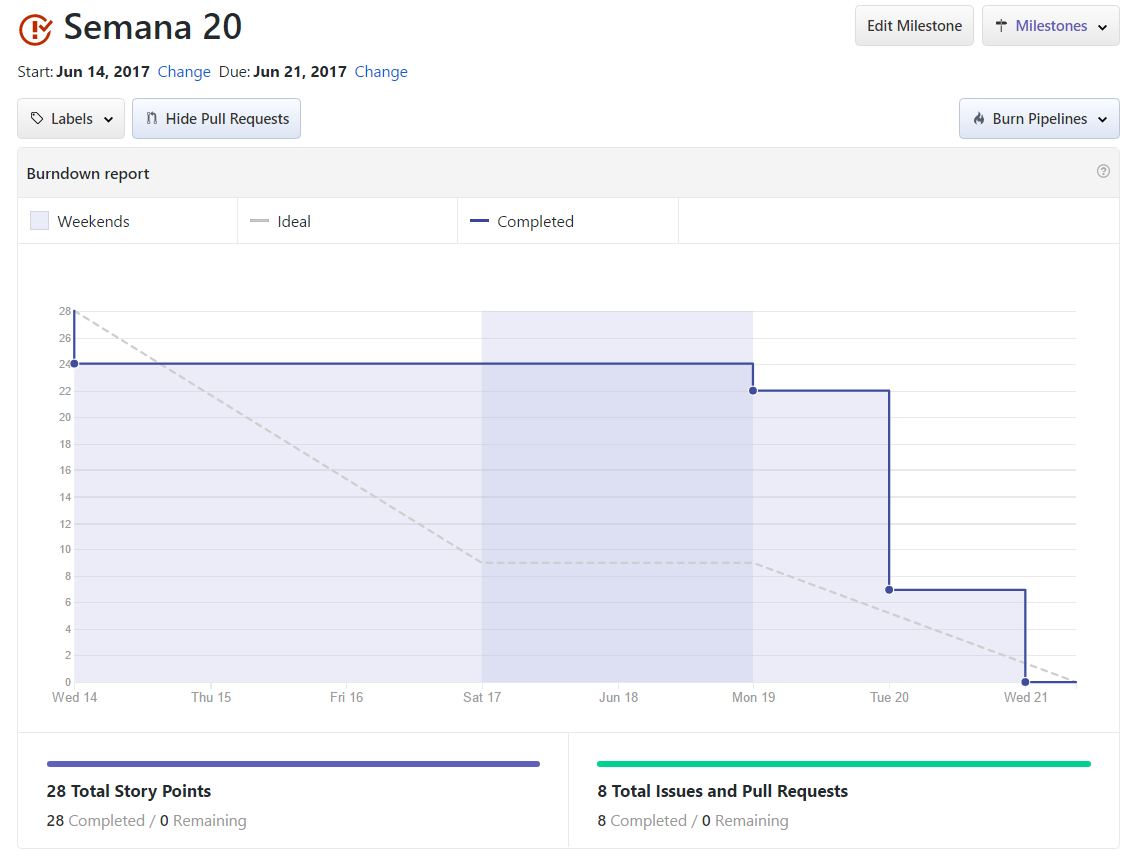
\includegraphics[width=0.99\textwidth]{Semana20}
\caption{Burndown del sprint 18.}
\label{fig:A.17}
\end{figure}

Hacemos además un cambio en el cifrado de las contraseñas, siendo más rápido y sin posibilidad de recuperar la contraseña original. Se hace alguna comprobación de email, pero sin llegar asegurar que existe realmente. Se puede ver la gráfica aquí \ref{fig:A.17}.

\subsection{Sprint 19 (21/6/2017 - 28/6/2017)}

Para terminar, en el último \emph{sprint} a parte de documentar todo lo que falta, tenemos que solucionar pequeños errores y hacer el despliegue de la aplicación.

Las tareas son:
\begin{itemize}
\item Desplegar la aplicación.
\item Solucionar un \emph{bug} el borrado de la palabra en TASP.
\item Pruebas de istema sobre fallos.
\end{itemize}

\begin{figure}[h]
\centering
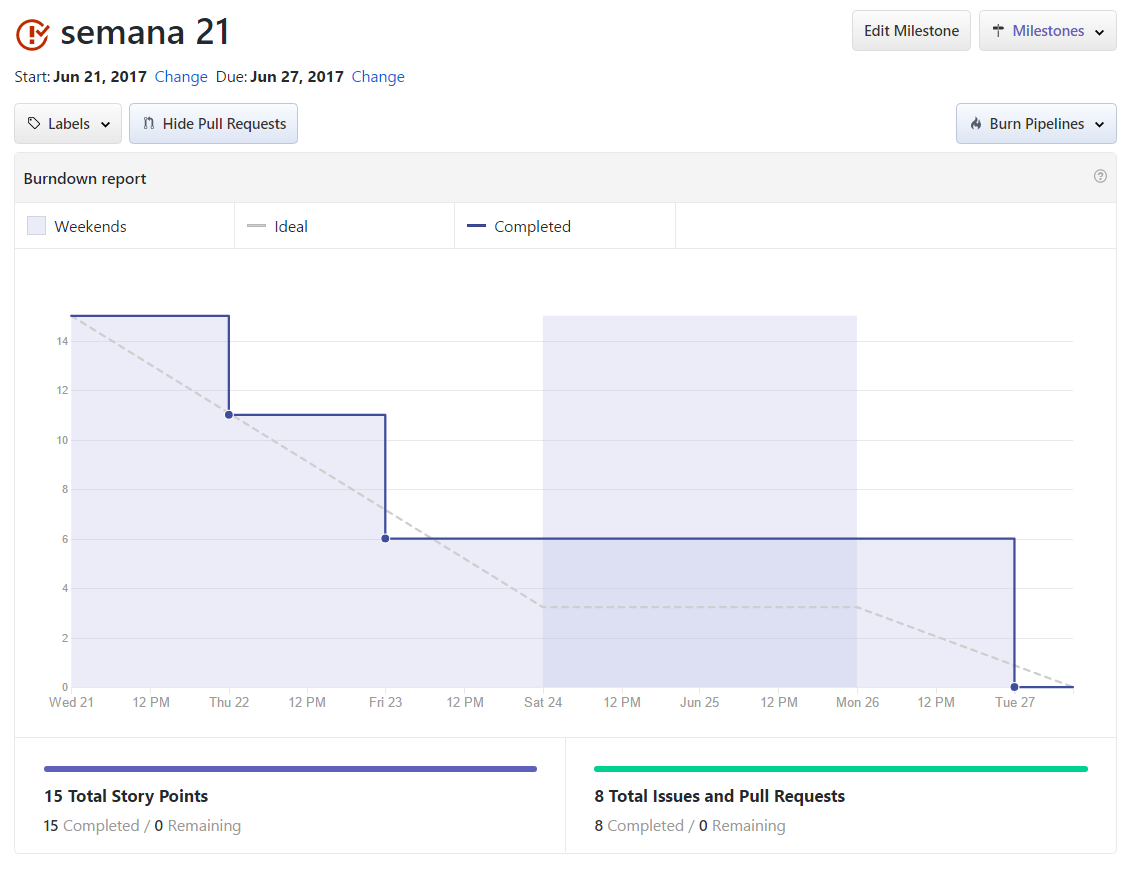
\includegraphics[width=0.99\textwidth]{Semana21}
\caption{Burndown del sprint 19.}
\label{fig:A.18}
\end{figure}

A parte de las pruebas para comprobar que el inicio de sesión también probamos que se producen errores cuando deben producirse y debemos comprobar que los mensajes que se muestran son los indicados.

Logramos hacer el despliegue después de varios intentos, y es que en un principio pensamos hacerlo con un \emph{host} gratuito. Más tarde vimos que desde \emph{App Engine} se podía hacer de manera <<sencilla>>. Se puede ver el \emph{burdown char} aquí \ref{fig:A.18}.

\section{Estudio de viabilidad}

En este apartado se realiza un estudio de viabilidad del proyecto que consiste en utilizar la
técnica del análisis coste/beneficio. Con ello se obtiene una valoración de la justificación económica del proyecto.

El estudio de la viabilidad se divide en la
viabilidad económica y la viabilidad legal.
Para el estudio de viabilidad económica se supone que el proyecto ha sido realizado
dentro del ámbito empresarial. Quiere decir que se considera que los alumnos han recibido un sueldo por en base a la legislación por realizarlo.


\subsection{Viabilidad económica}

Para analizar la viabilidad económica, hay que tener en cuenta los constes de personal y los costes de material.

\subsubsection{Costes de personal}

Se cuenta como coste personal el trabajo del alumno, considerado como un programador junior. La duración del trabajo a sido de 5 meses, unos con más carga de trabajo que otros. Estimo unas 460 horas de trabajo y analizando un poco los sueldo de los programadores junior en Java que ronda los 9 euros la hora, el resultado es el siguiente.

\[ 460h * 9\textrm{\euro/h} = 4140\textrm{\euro}\]

A esto, debemos sumarle la Seguridad Social y otros impuestos que se deben pagar por empleado. En la actualidad, los costes a cargo de una empresa son los siguientes:

\begin{itemize}
\item Contingencias Comunes: 23,60\%
\item Desempleo de Tipo General: 5,50\%
\item Fondo de Garantía Social: 0,2\%
\item Formación profesional: 0,6\%
\item \textbf{Total:} 29.9\%
\end{itemize}

Que esto equivale a un gasto por un trabajador de: 
\[ 4140\textrm{\euro} * 0,299 = 1237,86\textrm{\euro}\]
\subsubsection{Costes de material}

Como costes materiales se tienen en cuenta el software y el \emph{hardware}. El sistema operativo es Windows versión 8.1 Home, que tiene un precio de 45\euro{} A parte de esto, el software es completamente gratuito y no necesita ninguna licencia bajo pago. La plataforma \emph{Google Cloud}, es gratis durante el primer año y la licencia caduca el 26 de junio de 2018. Además de regalo tengo 300 dólares a gastar en dos meses de servicios. En cuanto al \emph{hardware} tendremos en cuenta el equipo en el cual se ha desarrollado. Se trata de un computador con un valor de 980\euro, que teniendo en cuenta su amortización media de unos 5 años de uso, el cálculo sería el siguiente. 
\[ \frac{980\textrm{\euro}}{12\textrm{meses} * 5 \textrm{periodos}} *5\textrm{meses de uso} = 81,66\textrm{\euro}\]
 
Por lo tanto los costes totales quedaría reflejados en la tabla \ref{tab:costes}.

\begin{table}[]
\centering
\rowcolors {2}{gray!35}{}
%\resizebox{0.5\textwidth}{!}{
\begin{tabular}{p{4cm} r}
\toprule
Costes & Importe \euro{} \\ \midrule
Personal         & 4140   \\ 
Seguridad Social & 1237,86 \\ 
Material         & 126,66  \\ 
\textbf{Total}   & \textbf{5504,52} \\ \bottomrule
\caption{Tabla de los costes totales}
\label{tab:costes}

\end{tabular}
%}
\end{table}

\subsection{Viabilidad legal}

En el marco de la viabilidad legal, se debe considerar las licencias de los programas y librerías utilizados para la realización de la aplicación.

Para el desarrollo del proyecto se ha hecho uso del \emph{framework} GWT, que cuenta con la Licencia Apache 2.0, que es una licencia software libre permisiva compatible con GPL y aprobada por la \emph{Open Source Initiative}. Esto se traduce en que el software producido bajo los términos de esta licencia otorga a usuario la utilización del software para cualquier propósito de modificación o distribución.

Las librerías que se emplean también son gratuitas y de código abierto, como se puede observar en la siguiente tabla~\ref{tabla:Licencias}. 

\begin{table}[]
	\centering

	\rowcolors {2}{gray!35}{}

	\begin{tabular}{@{} p {.25\textwidth} p {.1\textwidth}@{} p {.40\textwidth} p {.25\textwidth}@{} }
	\toprule
	Librería     & Versión & Descripción & Licencia\\
	\midrule
	App Engine SDK for Java      & 1.9.34     &  Conjunto de librerías para trabajar con la plataforma App Engine. & Apache License 2.0
	\\ 	
	GWT SDK     & 2.7.0  &  Contiene las librerías principales y el compilador que se necesitan para escribir aplicaciones web. & Apache License 2.0  
 	\\ 	
	JRE System Library        & 1.8.0-60  & Contiene las librerías mínimas de Java para ejecutar la aplicación. & 
	\\ 	
	JUnit & 0.12.3  & Framework que sirve para hacer pruebas de sistema.	               & Eclipse Public License 1.0
	\\ 	
	Google Plugin     & 3.9.6    & Sirve para desarrollar utilizando GWT y despliega aplicaciones en el entorno de App Engine. & Eclipse Public License v 1.0
	\\ 	
	Google App Engine Maven Integration       & 3.9.6   & Una herramienta de gestión de proyectos de software. & Eclipse Public License 1.0
	\\ 
	ObjectAid Class Diagram        & 1.1.14   & Herraminta de visualización de código y creación de diagramas para Eclipse. & Eclipse Public License v 1.0
               \\ \bottomrule
\end{tabular}
	\caption{Tabla de software y sus licencias}
	\label{tabla:Licencias}
\end{table}


\apendice{Especificación de Requisitos}

\section{Introducción}

En esta sección se definirán los requisitos de la aplicación así como los objetivos de una forma más esquemática y concreta que en otros apartados. De esta manera se puede ver en que dirección va orientado el proyecto y porque se ha elegido cada uno de acuerdo a los requisitos.

\section{Objetivos generales}

Estos has sido los principales objetivos del proyecto según la línea de tiempo.

\subsection{Crear un prototipo de aplicación cliente-servidor con GWT}

El objetivo de crearlo es el de poder ver el funcionamiento, comunicación y procesado del lenguaje Java en GWT para definir que limitaciones y posibilidades de un proyecto realizado con esta herramienta. Con ello se define que:  
\begin{itemize}
\item El lado del cliente y el compartido (shared) son los que se traducen al lenguaje JavaScript y los ficheros se crean dentro de un directorio <<war>>.
\item El lado del cliente tiene ciertas limitaciones y no acepta todo tipo de librerías de Java. 
\item La comunicación entre cliente y servidor es por medio de llamadas de procedimiento remoto o RPC.
\item Parte de la aplicación debe ir indudablemente en el servidor y comunicarse con el cliente para mostrar los resultados 
\end{itemize}

Este primer objetivo es fundamental y marca las posibilidades reales que ofrece GWT de cara a este proyecto.

\subsection{Construir la aplicación con la definición de gramática}

Consiste en hacer ya el comienzo de la aplicación empezando por la <<definición de gramática>> que es la parte de Thoth en la que se introduce un a gramática en un recuadro de texto y el programa es capaz de identificarla y mostrar sus propiedades. Para ello es necesario haber logrado en objetivo anteriormente descrito, ya que se necesita alojar en el servidor el <<parser>> de la gramática y hacerle peticiones desde el cliente para interpretarla y mostrar sus propiedades.

Es el comienzo de la aplicación y la base sobre la que trabajar posteriormente ya que para implementar los algoritmos es necesario tener definida una gramática.

\subsection{Construir los algoritmos sobre gramáticas}

El objetivo es implementar cada unos de los algoritmos que se aplican sobre una gramática en Thoth. Es una de las utilidades más importantes de esta aplicación y la cuál otorga mas posibilidades a los usuarios. Esta compuesta por los algoritmos siguientes:

\begin{itemize}
\item Eliminación de símbolos no terminales.
\item Eliminación de símbolos no alcanzables. 
\item Eliminación de símbolos anulables.
\item Eliminación de producciones no generativas.
\item Eliminación de recursividad directa.
\item Eliminación de recursividad indirecta.
\item Factorización por la izquierda.
\item Forma normal de Chomsky.
\item Análisis descendente LL(K) formado por el cálculo de <<First y Follow>> y reconocimiento por medio de TASP o Tabla de Análisis Sintáctico Predictivo.
\end{itemize}

Hay además dos funcionalidades que engloban varios de estos algoritmos como son la de limpiar gramática y eliminar recursividad.

Varois de ellos tienen la particularidad de que su ejecución esta hecha paso a paso, señalando dichos pasos con un resaltado con colores.

\subsection{Construir un registro de usuarios}

Es el objetivo puesto en último lugar debido a que la prioridad principal era que la aplicación funcionase correctamente y una vez conseguido añadir funcionalidades asociadas a ella. Consiste en, por medio de la aplicación cliente-servidor, hacer una base de datos con los usuarios que se conecten a la aplicación una vez que hayan sido registrados.

Se comprueba que los datos introducidos cumplen una serie de requisitos y se debe rellenar una información que se almacena en la base de datos.
El fin de este registro es para obtener información de quienes accedan a la aplicación y poder así analizar por ejemplo cuantos usuarios han hecho uso de ella.

\section{Catalogo de requisitos}

\section{Especificación de requisitos}



\apendice{Especificación de diseño}

\section{Introducción}
En esta sección se habla sobre la fase de desarrollo software en la que definen la arquitectura, los procedimientos o los datos que se utilizan. 

\section{Diseño de datos}

\section{Diseño procedimental}

\section{Diseño arquitectónico}



\apendice{Documentación técnica de programación}

\section{Introducción}

En esta sección se hablara de aspectos más técnicos pensando en futuros desarrollos. Sirve como ayuda para entender el funcionamiento de la aplicación y de los pasos que se han llevado a cabo para conseguir estos resultados. Se habla de la estructura del programa, de la instalación y configuración de las herramientas necesarias y del proyecto y, por último, de las pruebas realizadas.

\section{Estructura de directorios}


\subsection{Aplicación}
Dentro se encuentra la carpeta \textbf{Thoth-Web}. En este directorio se almacenan los fichero del código fuente del proyecto en src, el directorio war, y también los test.

\begin{itemize}
	\item src
		\begin{itemize}
			\item client
			\item shared
			\item server
			\item módulo Login
			\item módulo GramaticaCS
		\end{itemize}
	\item test
		\begin{itemize}
			\item login
			
		\end{itemize}
	\item war
		\begin{itemize}
			\item imagenes
			\item login
			\item gramaticacs
			\item WEB-INF
		\end{itemize}
\end{itemize}	

Client esta organizado de la siguiente manera:

\begin{itemize}
	\item algorithms
	\item core
	\item gui
	\item login
	\item register
	\item main
	\item archivos de comunicación con el servidor
\end{itemize}	

Server contiene los siguientes elementos:
\begin{itemize}
	\item RegServlet.java
	\item GrammarServiceImp.java
	\item SessionServlet.java
\end{itemize}
\subsection{Prototipos}

En este directorio, se encuentran los prototipos hechos al inicio del proyecto. Sirven para entender el funcionamiento de diferentes aspectos de GWT como, creación de un proyecto, comunicación cliente-servidor y dos pruebas con el núcleo de Thoth cliente-servidor.

\begin{itemize}
	\item CorePrueba
	\item GWTProjectThree
	\item PrototipoCoreC-S
	\item StockWatcher
\end{itemize}	

\subsection{Documentación}

En este directorio se incluyen los la memoria y los anexos hechos con Latex, asi como las imágenes para documentarlos.

\section{Manual del programador}

\subsection{Instalación y configuración de GWT:}


Para poder trabajar con GWT \footnote{\url{http://www.oracle.com/technetwork/java/javase/downloads/index.html}}, se debe descargar el SDK de GWT proporcionado en la página web oficial. Los requisitos previos para crear un aplicación web con Google Web Toolkit son básicamente dos: tener instalada la SDK de Java en su versión 1.6 o cualquiera superior a esta y tener instalado también Apache Ant o en su defecto Apache Maven.

En mi caso, como trabajo con la plataforma Eclipse (versión 4.4.) al descargar el plugin de Google para Eclipse, este viene con GWT y la App Engine SDK, todo junto. Se puede descargar desde la siguiente dirección \footnote{\url{http://www.gwtproject.org/usingeclipse.html}}.

Para instalar el plugin desde eclipse, solo tenemos que ir a <<help>> y en el desplegable elegir la opción <<Instal new software>>. Aparecerá una ventana con un recuadro en el que pone <<work with>> y nos da la opción de escribir una dirección web. Para consultar las direcciones según la versión de Eclipse sólo tiene que visitar \url{https://developers.google.com/eclipse/docs/download}.
Aparecerá los elementos que se pueden instalar, y ahí elegimos el plugin de Google. Debemos esperar a que se instale y ya solo hará falta reiniciar Eclipse.

Como último paso, se debe referenciar la SDK de GWT y completar la instalación. Para habrá que ir a la opción <<window>> de la pantalla principal, hacer click en preferencias y aparecerá una ventana con varias opciones. Buscamos la opción de Google y en <<web toolkit>> y ahí añadir la referencia a la SDK con la dirección en la que se encuentra el archivo. Lo mismo hay que hacer para el <<App Engine>> pero en este caso añadiendo la referencias al App Engine.

El modo de trabajar con GWT es muy simple. Desde el plugin podemos crear un nuevo proyecto dese <<New Web Application Project>>, darle un nombre y marcando las opciones del SDK y el App Engine.

 
\subsection{Parser JavaCC}

GWT esta compuesto por una parte cliente, que es la que será traducida a JavaScript, y otra servidor escrita en Java y que no se traducirá. En un principio se prueba a incluir toda la aplicación dentro del lado del cliente, traduciendo todo a JavaScript. Pero como ya se ha dicho en otros apartados, GWT sólo soporta unas determinadas librerías en dicho lado y tiene algunas restricciones más\footnote{\url{http://www.gwtproject.org/doc/latest/DevGuideCodingBasicsCompatibility.html}.} que obligan a incluir el parser de JavaCC en el servidor, en vez del cliente.

Originalmente en el núcleo de Thoth, dentro del directorio <<grammar>>, colgaba un sub-directorio llamado <<parserjavacc>> en el cual se encontraba el parser para la gramática. Es la parte más importante a lo que a la gramática se refiere, ya que permite reconocer si una gramática está bien construida o no.


\subsection{Comunicación cliente-servidor}
Una vez alojado en el servidor el parser habrá que establecer una comunicación entre la parte del ciente en la que habrá un método que llame a la funcionalidad que se desee del servidor.

Para hacerlo, GWT utiliza la técnica denominada por sus siglas en inglés RPC o llamada de procedimiento remoto (Remote Procedure Call) que tiene una estructura similar a la siguiente ilustración \ref{fig:5.1}.

\begin{figure}[h]
\centering
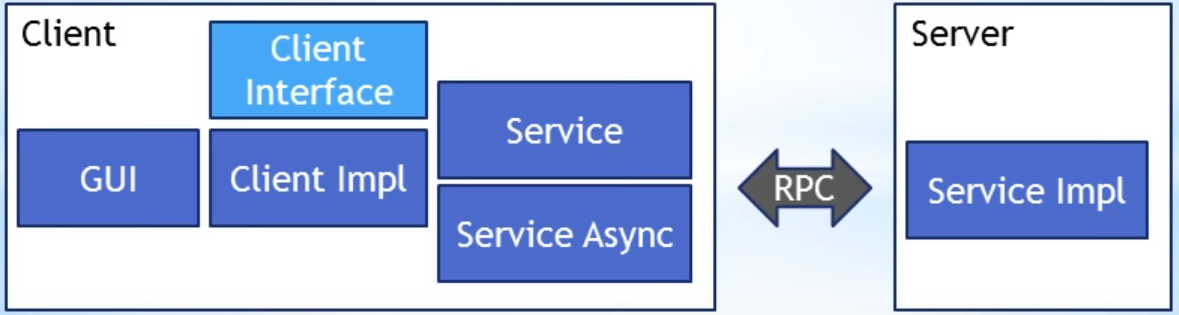
\includegraphics[width=0.65\textwidth]{RPC}
\caption{Arquitectura RPC simple. Fuente propia.}
\label{fig:5.1}
\end{figure}

Del lado del cliente tenemos, en este caso, una interfaz gráfica de usuario (GUI), una clase dedicada a hacer las llamadas RPC (ClienImpl), dos interfaces que definen los métodos (Service y ServiceAsync), una clase con los métodos en el lado del servidor (serviceImpl) y por último una interfaz, que no es esencialmente necesaria (ClientInterface). 

En términos generales, para utilizar el parser de la gramática, que es quizá la clave de todo, hay que llamar al servidor y establecer una comunicación. Es ahí donde utilizamos la clase <<GrmmarServiceClientImp>> que hace las llamadas a las interfaces necesarias hasta llegar al servidor. Esta clase es un nexo de unión entre la parte del núcleo, que ese encuentra en el servidor, y la parte del cliente, que contiene lo visual y las acciones de los botones entre otros. La comunicación queda representada en este diagrama\ref{fig:5.2}.

\begin{figure}[h]
\centering
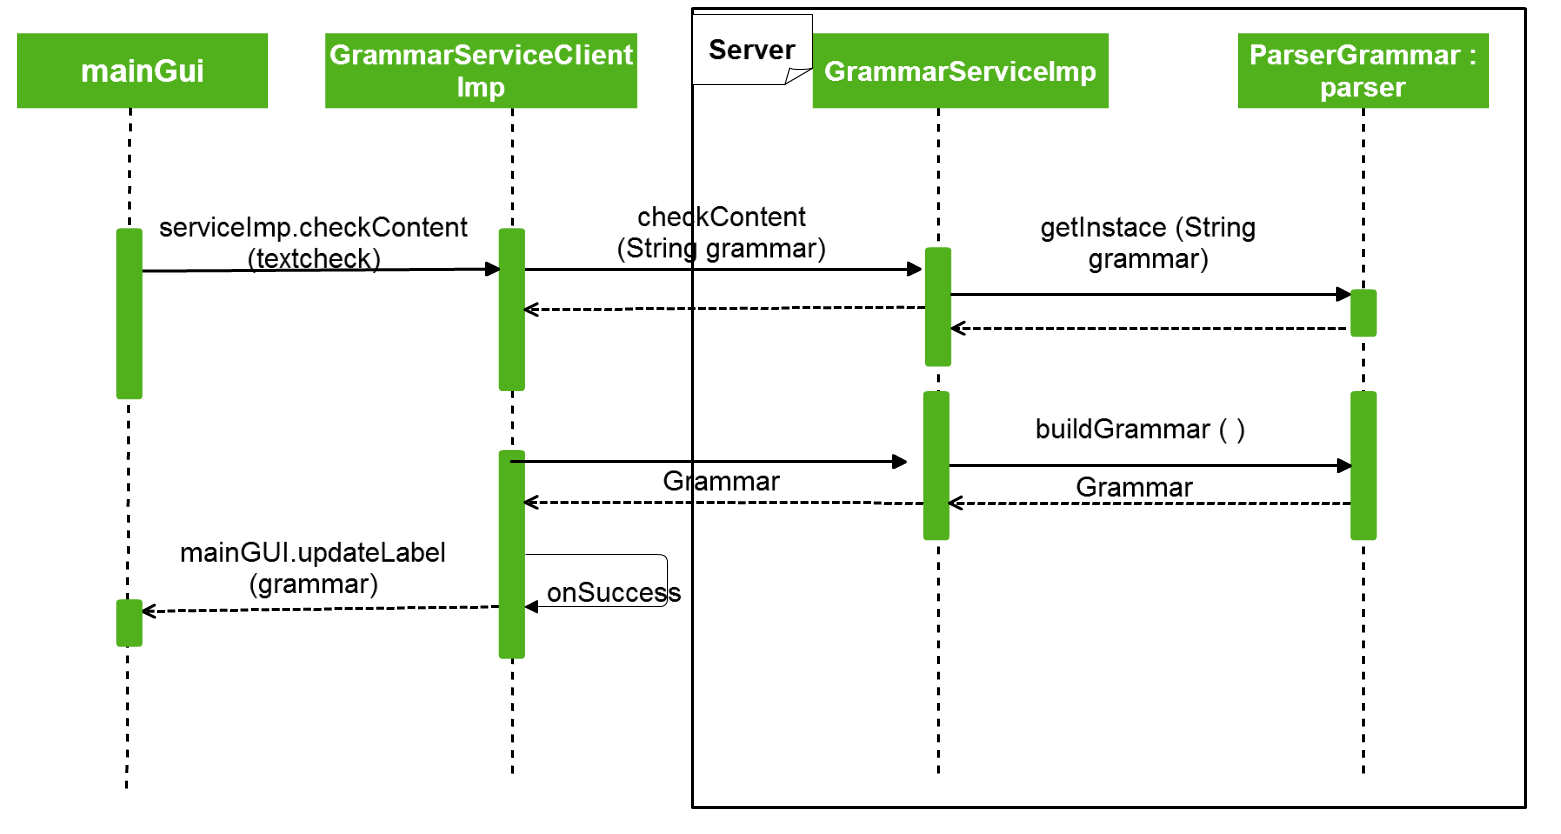
\includegraphics[width=1.1\textwidth]{ParserDiagram}
\caption{Diagrama sobre la comunicación entre el cliente y el servidor en GWT.}
\label{fig:5.2}
\end{figure}

Dentro de la clase <<GrammarServiceClientImp>> hay tres constructores según le pasemos una gramática, un texto, simplemente nada. El atributo url es simplemente la localización del <<servlet>> que se utiliza para la comunicación RPC. Estos detalles se aprecian mejor en el diagrama de clases que muestra la siguiente imagen \ref{fig:5.3}.

\begin{figure}
\centering
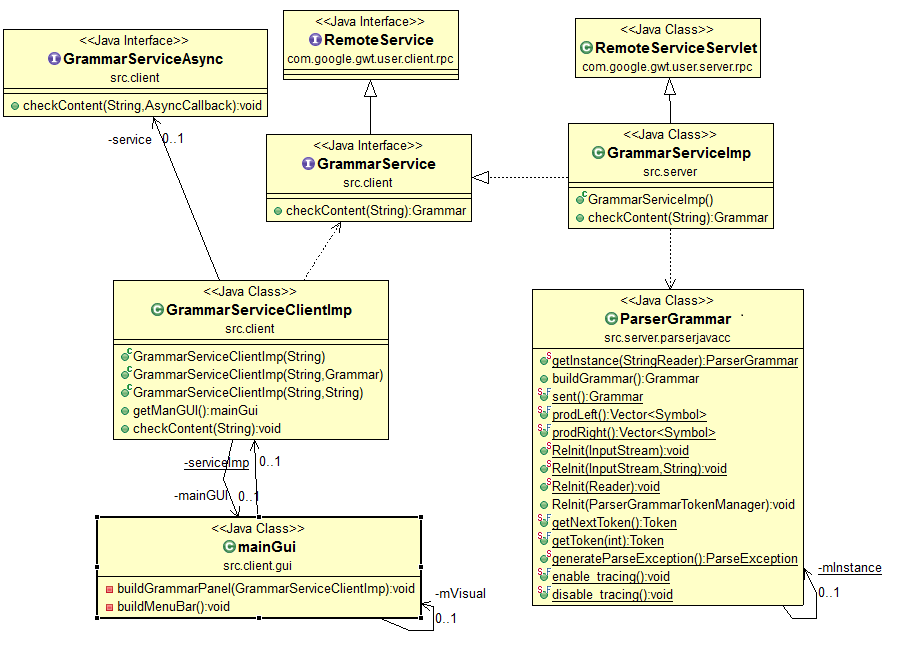
\includegraphics[scale=0.9]{Parser-ClassDiagram}
\caption{Diagrama de clases que muestra como utiliza el parser de la gramática. Diagrama realizado con ObjectAid.}
\label{fig:5.3}
\end{figure}

Una vez hechos todos estos pasos, es posible que no funciona nada, es más, dará un error del tipo \textit{did you forget to inherit a required module?}. Todos los errores parecidos a este tienen que ver con el archivo <<web.xml>> que se encuentra en todos los proyectos GWT dentro de la carpeta <<war>> en <<WEB-INF>>. En ese archivo tenemos que definir los <<servlets>>, dándolos un nombre y especificando la dirección, dentro del proyecto, donde se encuentran. Después deberemos indicar la dirección del patrón, es decir indicar a que módulo pertenecen y con que nombre. Ese nombre se lo especificamos anteriormente en la interfaz <<GrammarService>> con el componente <<@RemoteServiceRelativePath(``nombre'')>>.

\section{Compilación, instalación y ejecución del proyecto}

Antes de empezar a hablar sobre compilación debemos contar con un proyecto en GWt, preferiblemente en Eclipse, habiendo instalado el pluguin de Google, el SDK de App Engine para Java y el SDK de GWT.

Hace unos años Google contaba con un plugin para algunos navegadores (Chrome y Firefox, no confundir con el plugin de Eclipse) con los que se podía ejecutar el proyecto. Pero Google paró el mantenimiento. Afortunadamente los desarrolladores de GWT crearon <<GWT Super-Dev Mode>> que permite ejecutar cualquier proyecto realizado con esta herramienta.

En la definición del módulo, para poder realizar la ejecución con <<Super-Dev Mode>> debemos incluir la sentencia \textit{add-linker name=``xsiframe''}. Si no lo incluimos podemos incurrir en algún tipo de error al ejecutarlo.
Las definiciones de los módulos se encuentran en la raíz de la carpeta principal y tienen una extensión <<.gwt.xml>>. Es habitual que no se llegue a hacer la compilación porque no se han definido los servlets dentro del archivo <<web.xml>>.
  
\begin{figure}
\centering
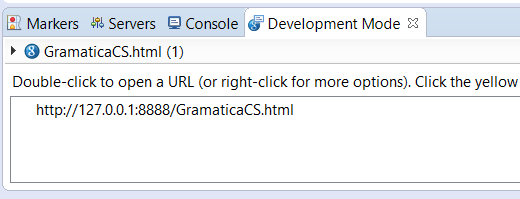
\includegraphics[scale=0.7]{SuperDevMode}
\caption{Dirección local que aparece al ejecutar en modo SuperDevMode.}
\label{fig:5.4}
\end{figure}

De esta forma una vez que se haya ejecutado en eclipse, se mostrará una dirección local que podemos abrir en nuestro navegador\ref{fig:5.4}. Este compilara los archivos HTML, y los JavaScript. Este proceso tardará unos segundo y cuando termine se mostrará la aplicación.

Si tenemos una base de datos, para poder acceder a ella, hay que coger la raíz de la dirección local, en nuestro caso <<http://127.0.0.1:8888/>>, y añadirle <<\_ ah/admin>>. Desde ahí podemos ver las entidades que hay, y en cada una de ellas los datos almacenados.


Por otro lado podemos desplegar la aplicación en App Engine. Seleccionamos el proyecto que queramos, y nos vamos al plugin de Google donde hacemos click en <<Deploy App Engine>> como muestra la imagen\ref{fig:5.5}. A continuación debemos dar un nombre al proyecto y en <<App Engine project settings...>> especificamos el identificador. Para hacerlo, debemos crear una cuenta aquí\footnote{\url{https://console.cloud.google.com/appengine}} y crear un proyecto. Automáticamente se le asignara un ID y ese es el que debemos introducir\ref{fig:5.6}. 
\begin{figure}
\centering
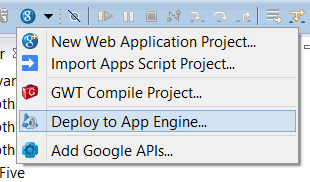
\includegraphics[scale=0.6]{Desplegar}
\caption{Acción de desplegar la aplicación con App Engine.}
\label{fig:5.5}
\end{figure}

\begin{figure}
\centering
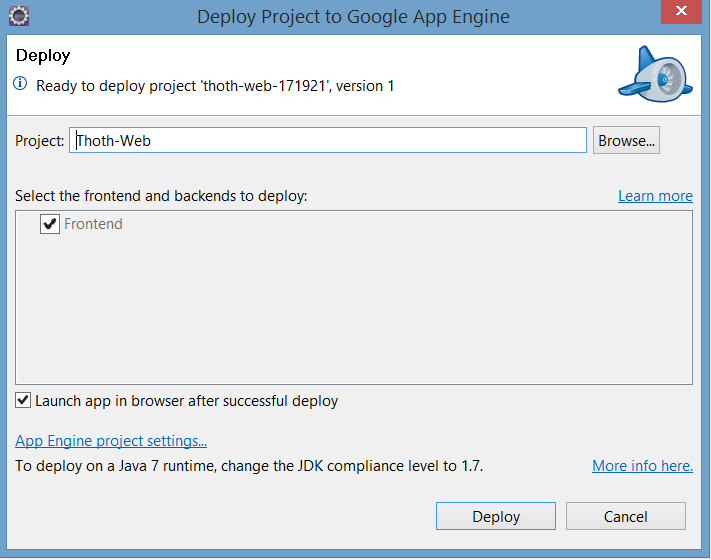
\includegraphics[scale=0.7]{Desplegar-dos}
\caption{Opciones de despliegue.}
\label{fig:5.6}
\end{figure}

Es importante que el SDK de Java sea el 1.7 ya que de lo contrario se producirá un error y no se desplegará la aplicación. La operación tardará un tiempo y ya solo quedará ir a la plataforma y ver si todo ha salido correctamente.

Si todo ha sido correcto, desde la nube podemos acceder a la base de datos como hacíamos en modo local, incluso con más detalle.

\section{Pruebas del sistema}


Las pruebas de sistema las hemos realizado con ayuda de Selenium \footnote{\url{http://www.seleniumhq.org/}}. Selenium es un entorno para realizar pruebas software en varios lenguajes, entre ellos, Java. Esta pensado para utilizarse en aplicaciones web. Para ello se puede descargar una extensión para el navegador, que digamos, grabará los pasos para cada test. Con esto se logra comprobar que el funcionamiento es correcto.

En este proyecto, hemos hecho pruebas de inicio de sesión
\apendice{Documentación de usuario}

\section{Introducción}

En este apéndice se van a mostrar los requisitos, la instalación y un manual para que el usuario final pueda manejar la aplicación de forma fluida. Para ello se ilustrará con figuras que muestren los detalles de los procesos.

\section{Requisitos de usuarios}

Los requisitos por parte del usuario son mínimos. No es necesario descargarse nada, ni hacer ninguna instalación así que en cuanto a software lo único que necesitará es un sistema operativo común y navegador web actual. Las versiones de compatibles son prácticamente la mayoría.

\begin{itemize}
    \item Firefox.
    \item Internet Explorer 8, 9, 10, 11
    \item Safari 5, 6
    \item Chromium y Google Chrome.
    \item Últimas versiones de Opera.
\end{itemize}

En cuanto a los requisitos hardware, es necesaria un equipo con conexión a Internet. No hay requisitos mínimos de procesador o memoria. 

La única petición que se le hace al usuario es la de proporcionar unos datos de registro que constan de un nombre con sus apellido, un correo electrónico y una contraseña.  

\section{Instalación}

El proyecto no requiere la instalación de ningún software adicional.

\section{Manual del usuario}

Una vez cumplamos tengamos un navegador y conexión a Internet ya podemos comenzar a usar la aplicación. Lo primero que tenemos que hacer es introducir la URL \url{https://1-dot-thoth-web-171921.appspot.com/gramaticacs/} en nuestro navegador. Ya habremos accedido a Thoth. Ahí como inicio nos aparece una ventana de inicio de sesión, como muestra la figura\ref{fig:6.1}.


\begin{figure}[h]
\centering
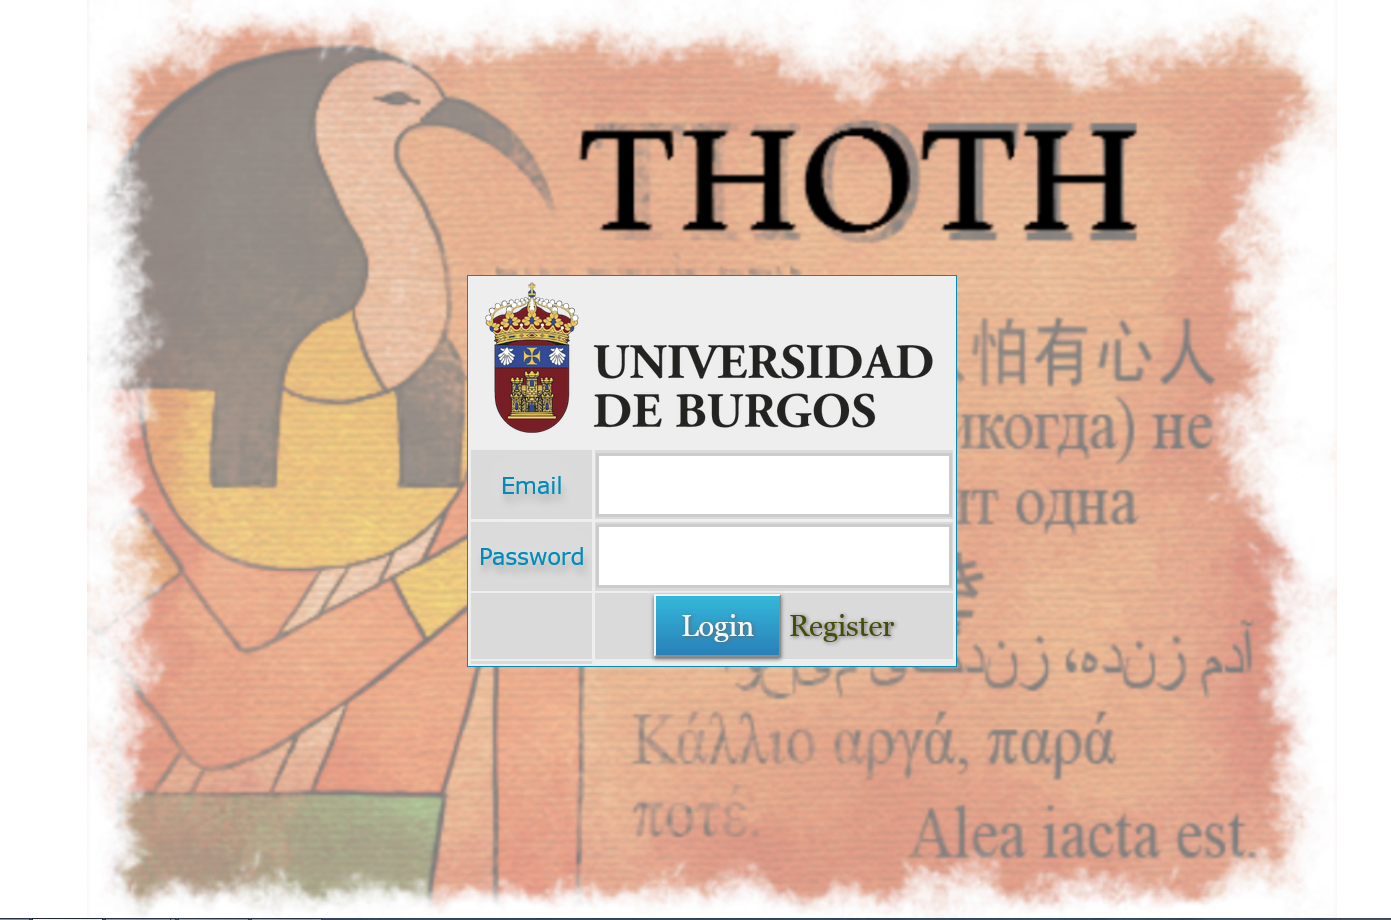
\includegraphics[width=0.50\textwidth]{Login}
\caption{Login en Thoth. Es lo que primero se ve al entrar en la aplicación.}
\label{fig:6.1}
\end{figure}

Al ser la primera vez que utilizamos Thoth no tendremos creada una cuenta, así que debemos registrarnos. Si pulsamos en el link <<Register>> aparecerá una vista con la siguiente pantalla\ref{fig:6.2}, en la que introduciremos los datos para crear una cuenta. Hay que tener en cuenta que los datos deben estar correctamente rellenados o de lo contrario, la aplicación nos mostrará un error del tipo <<Wrong fiel>>, campo incorrecto. Si el fallo es el correo electrónico, se marcará el campo en rojo\ref{fig:6.3}. En el caso de que el registro haya sido correcto, se mostrara un mensaje indicativo con el siguiente texto <<Registration Success>>.

\begin{figure}[h]
\centering
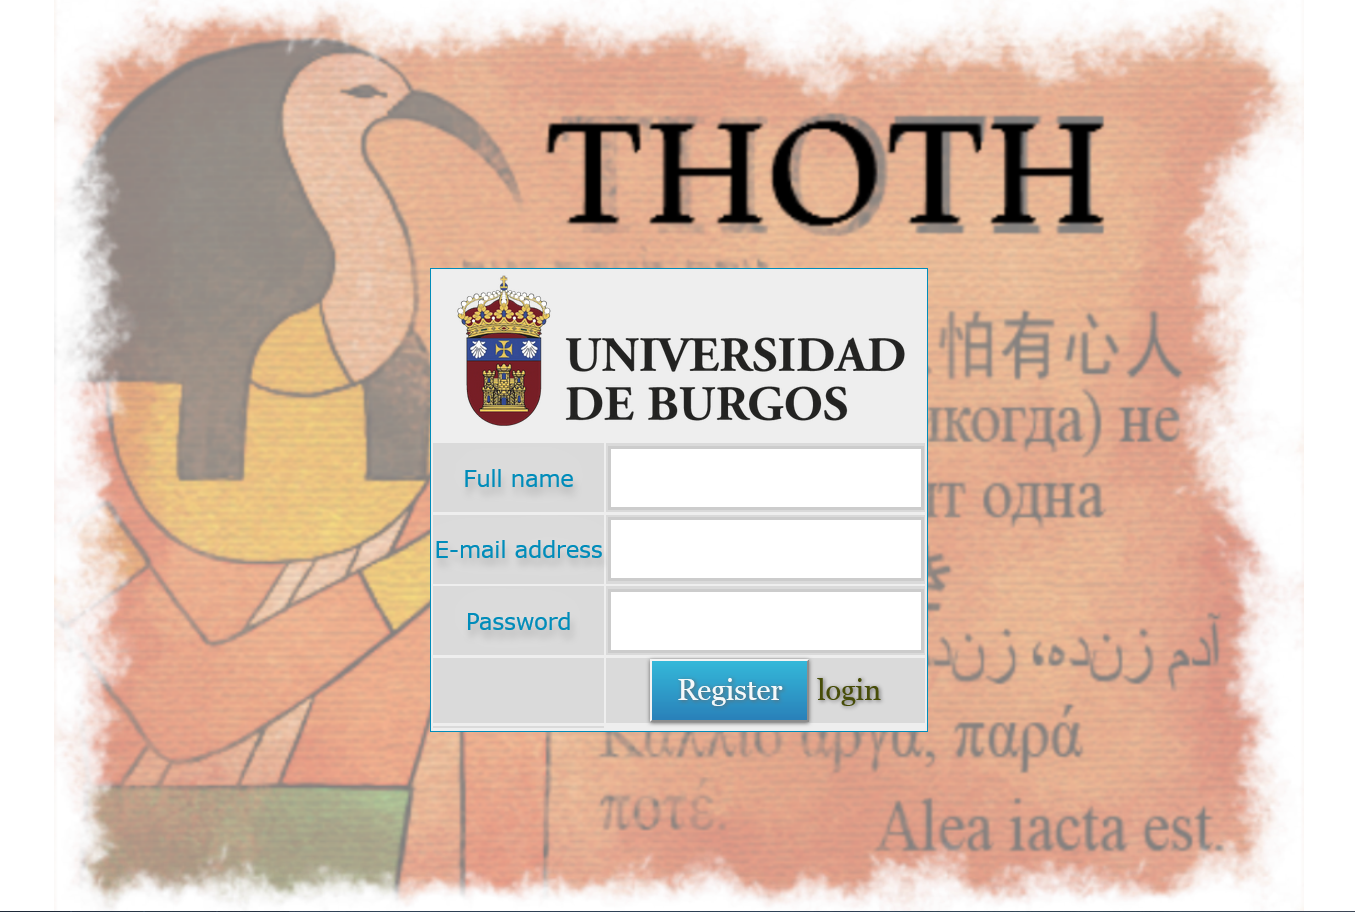
\includegraphics[width=0.50\textwidth]{Registro}
\caption{Pantalla de registro.}
\label{fig:6.2}
\end{figure}

\begin{figure}[h]
\centering
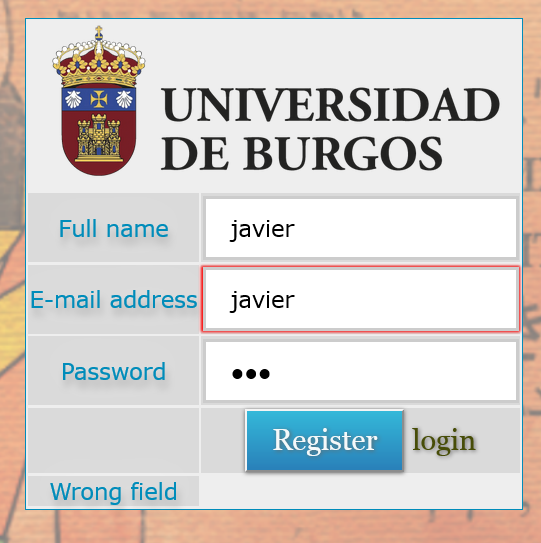
\includegraphics[width=0.40\textwidth]{Email-Error}
\caption{Fallo al introducir el email. Se muestra el campo en rojo.}
\label{fig:6.3}
\end{figure}

Una vez registrados, ahora sí, podremos iniciar sesión. Al hacerlo accedemos a la vista principal de la aplicación que consta de tres elementos principales. Un menú, en el que se despliegan diferentes opciones, un panel en el que introducir la gramática y por último una tabla con las características de la gramática. Esta vista se puede apreciar con detalle en la siguiente imagen \ref{fig:6.4}.


\begin{figure}[h]
\centering
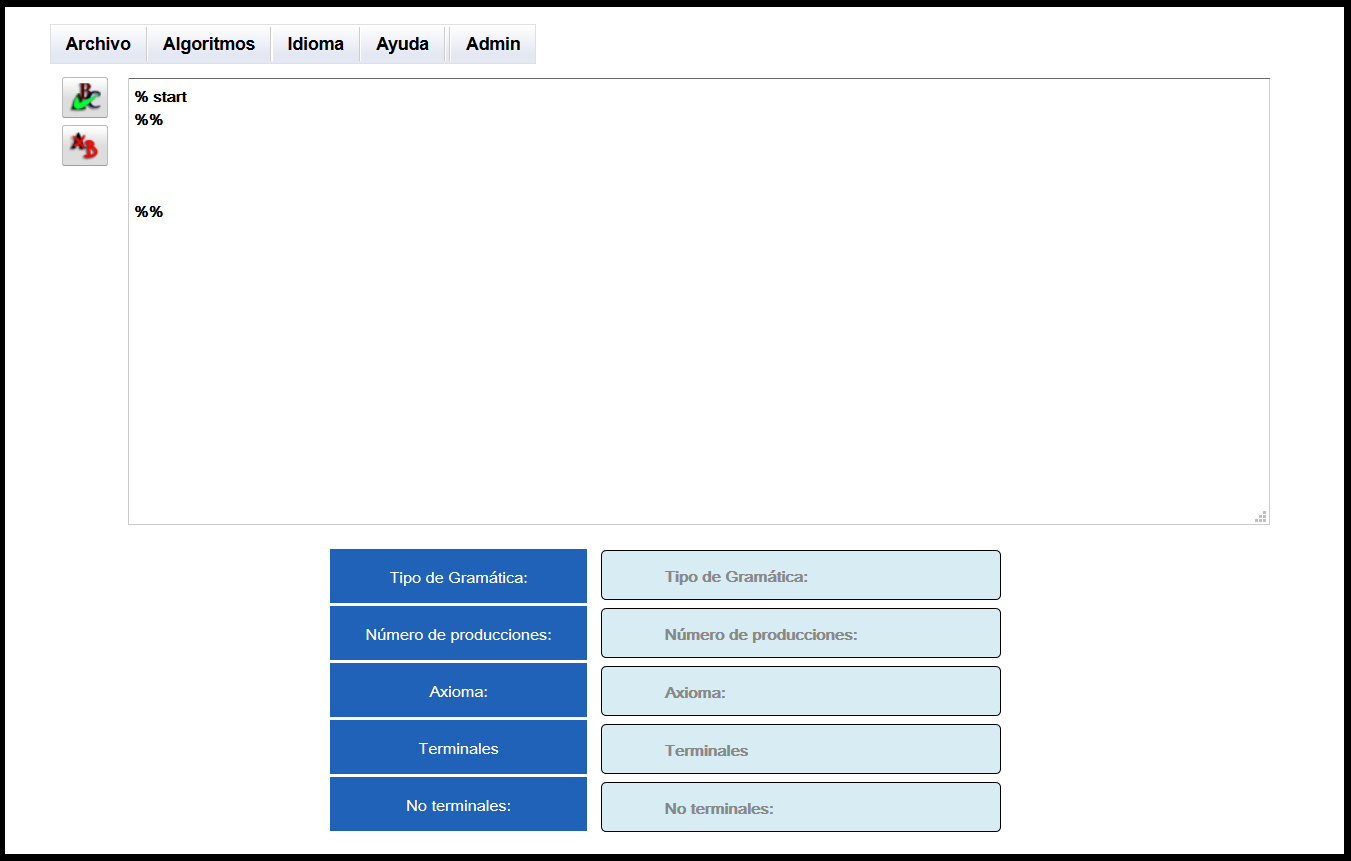
\includegraphics[width=1\textwidth]{Vista-Principal}
\caption{Pantalla principal con el menú de la aplicación y el panel para crear una gramática.}
\label{fig:6.4}
\end{figure}

La parte de azul claro es la que se actualizará, al comprobar una gramática, con las características de esta. Por defecto aparece qué característica es. También podemos apreciar como en el panel aparece ya algo escrito. Esto es para facilitar al usuario la labor al introducir la gramática de escribir ese comienzo. Las gramáticas que se leen en Thoth tienen siempre esa estructura. 

Para empezar, podemos centrarnos en la introducción de la gramática. En el panel podemos copiar, cortar, seleccionar y pegar cualquier carácter. Para comprobar una gramática solo tenemos que pulsar el botón de <<checkear>> en la parte superior. Por otro lado si queremos buscar y reemplazar un símbolo, el botón de renombrado aparece debajo\ref{fig:6.5}. 

\begin{figure}[h]
\centering

\includegraphics[width=0.1\textwidth]{botones-gramatica}
\caption{En la parte superior comprobar gramática y abajo renombrar. Ambos botones son los mismos que en las otras versiones de Thoth.}
\label{fig:6.5}
\end{figure}

Entonces, comenzamos introduciendo una gramática. En este caso los símbolos $\epsilon$ se representan con la letra E mayúscula y el símbolo \^. Comprobamos la gramática y en la parte inferior aparecen las características de esta \ref{fig:6.6}.  

\begin{figure}[h]
\centering
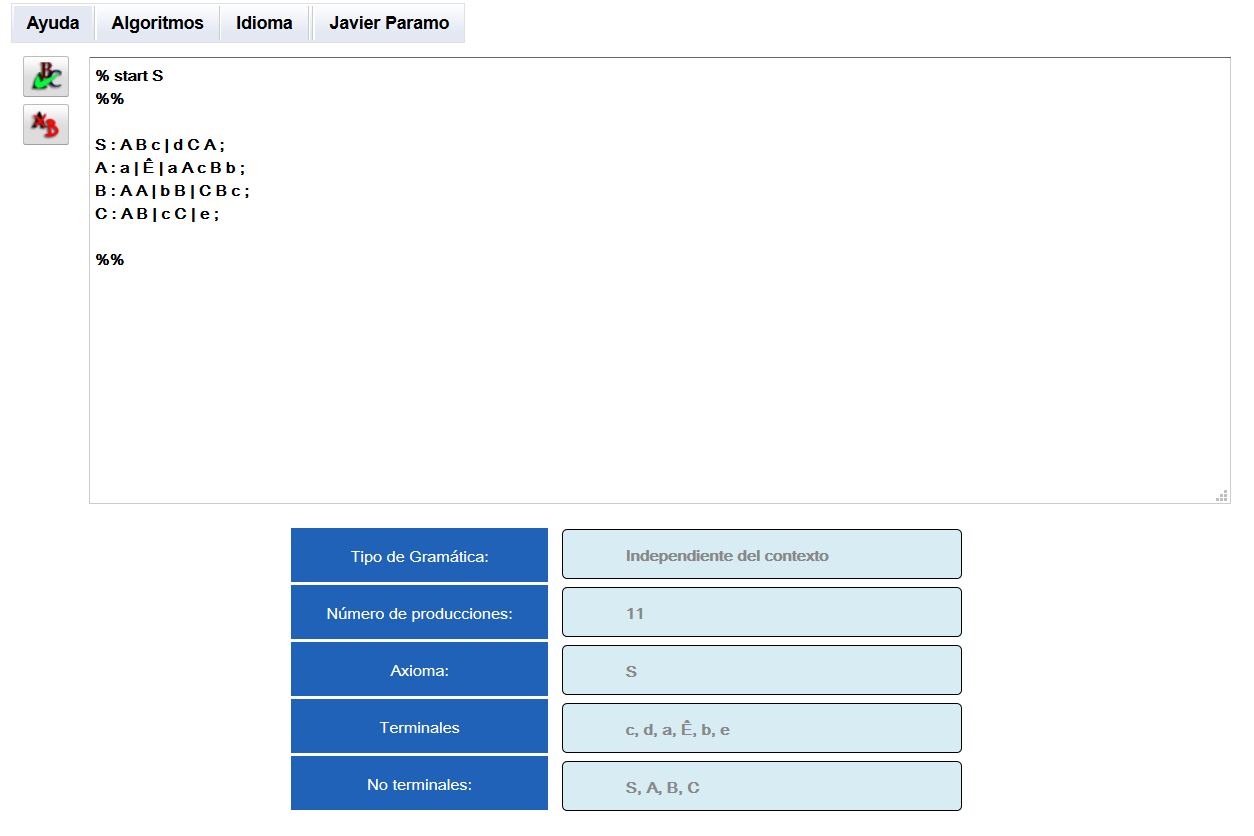
\includegraphics[width=1\textwidth]{comprobando-gramatica}
\caption{Comprobación de una gramática y como se actualiza la tabla inferior.}
\label{fig:6.6}
\end{figure}

Para renombrar aparecerá una ventana con esta forma\ref{fig:6.7}. En la parte superior introducimos el carácter a sustituir. Como se ve, aparece en forma de desplegable los caracteres iguale o similares. En la gramática es diferente la <<a>> que la <<A>>. Abajo se introduce el carácter que le sustituye.

\begin{figure}[h]
\centering
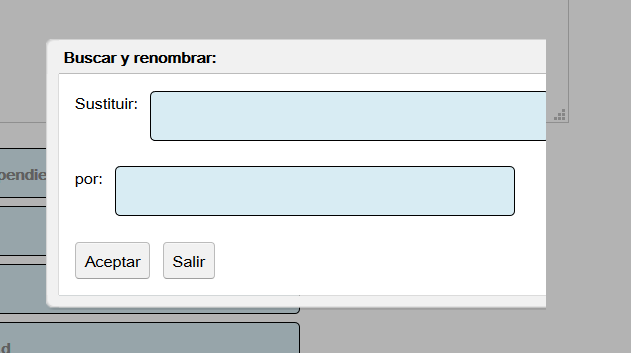
\includegraphics[width=0.40\textwidth]{Renombrado}
\caption{Renombrado de símbolos.}
\label{fig:6.7}
\end{figure}

Cuando se pulsa en aceptar se actualizará la gramática con la sustitución hecha. Entonces habrá que salir del panel.

Dentro de las opciones del menú, quizá la más utilizada es la de elegir uno de los algoritmos a aplicar a la gramática. En el desplegable se pueden ver todas las opciones que hay. Para no extendernos, mostraré las vistas de los algoritmos que sean diferentes a las demás. Antes de aplicar el algoritmo se debe comprobar la gramática, de lo contrario, la aplicación la comprobará automáticamente.

El algoritmo escogido es el de Eliminación de Símbolos Anulables como se puede apreciar en la imagen\ref{fig:6.8}. Es muy similar a los dos primeros algoritmos. Se puede apreciar como se resaltan las producciones en color verde y otras en rojo. Esto sólo ocurre cuando se aplica el algoritmo paso a paso. De lo contrario, no mostrará el proceso, y simplemente aparecerá a un lado la gramática antigua y al otro la nueva.

\begin{figure}[h]
\centering
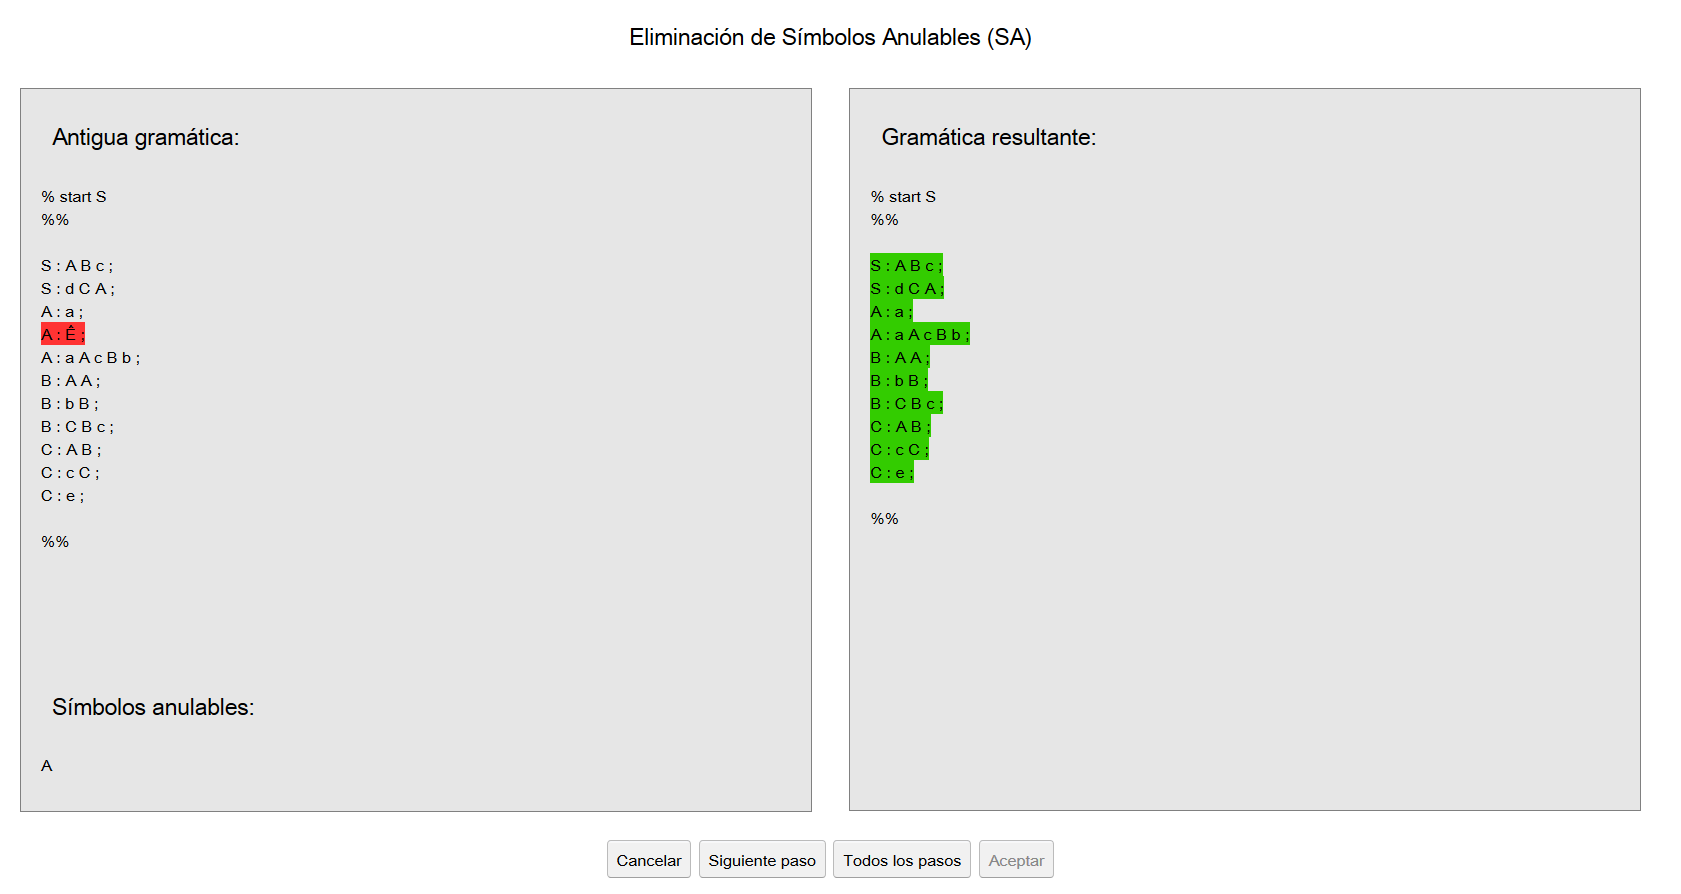
\includegraphics[width=1\textwidth]{vista-algoritmos}
\caption{Ejemplo de una vista del algoritmo Eliminación de SA.}
\label{fig:6.8}
\end{figure}

En verde se iluminan las producciones que pasan a la nueva gramática en ese paso, y en rojo se resalta el símbolo anulable que se está analizando. Si pulsamos en <<cancelar>> se vuelve a la vista principal de edición de gramática con la gramática antigua. Por el contrario se pulsamos en <<aceptar>> volveremos a la vista principal pero con la gramática resultante. El botón aceptar solo se activará una vez se haya terminado de aplicar el algoritmo, de lo contrario no tendría sentido. 

Los demás algoritmos tiene un <<modus operandi>> parecido, por lo que omitiré el proceso. Resaltar que tanto el algoritmo de Limpieza de Gramática como el de Eliminar Recursividad se aplican de forma directa. Es decir cuando se ejecutan no se pasa a una vista nueva, sino que se actualiza la gramática ya en el panel.

Los algoritmos que cambian bastante en la forma de proceder son l cálculo del First y el Follow y el reconocimiento por medio de TASP. El cálculo de First Follow deriva al reconocimiento con TASP, ya que ambos son algoritmos de análisis ascendente. En el ejemplo de First-Follow con cada botón se crea la tabla correspondiente\ref{fig:6.8}. Los botones de desactivan a mediada que se utilizan.

\begin{figure}[h]
\centering
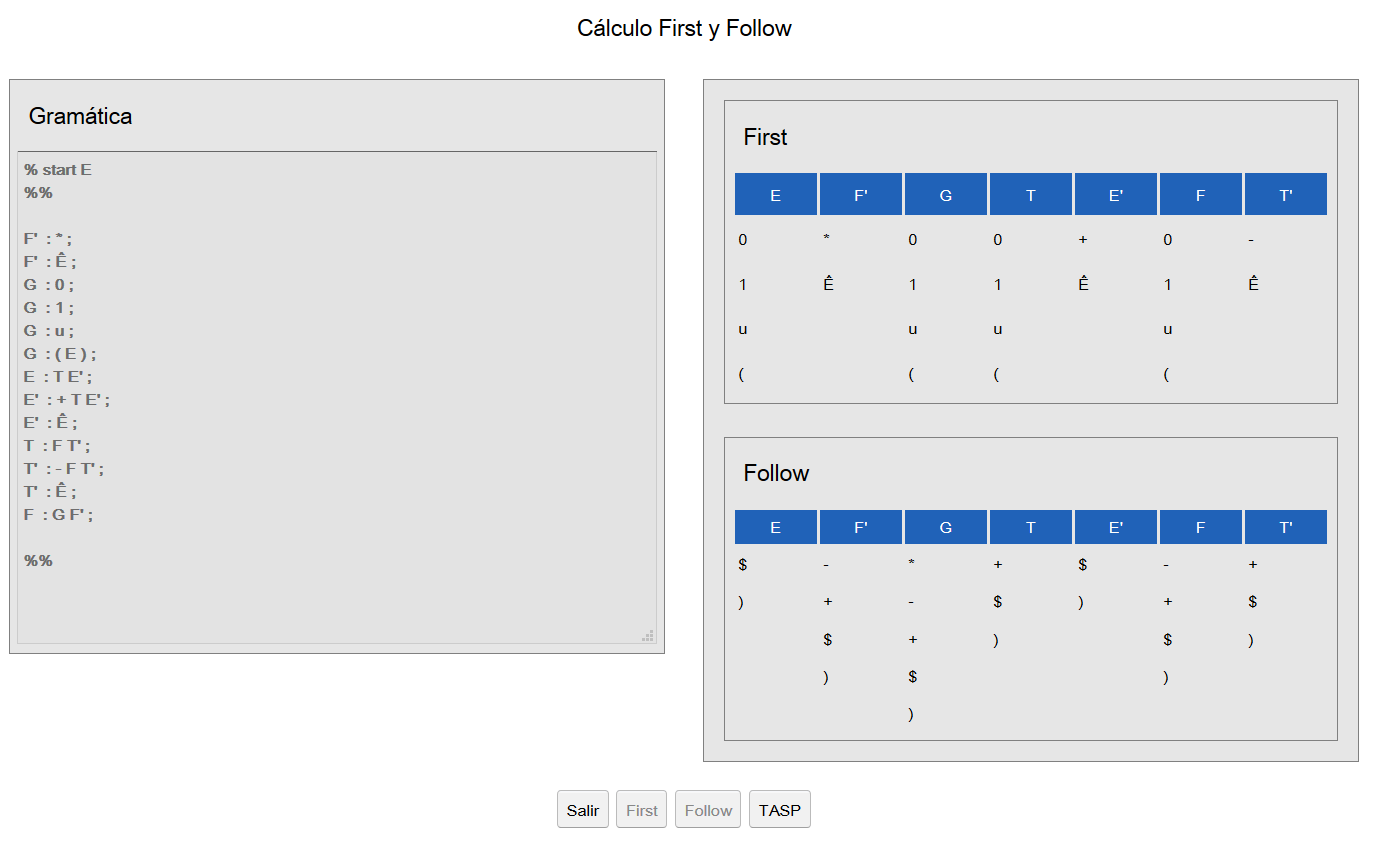
\includegraphics[width=1\textwidth]{calculo-ff}
\caption{Vista del algoritmo para el Cálculo de Fisrt Follow.}
\label{fig:6.9}
\end{figure}

Antes de ejecutar ambos algoritmos se pide confirmación adicional al usuario antes de proceder. Se conservan la forma de las anteriores versiones de Thoth. Como estos dos algoritmos no generan gramática nuevas no existe un botón de aceptar.

Para el reconocimiento con TASP, se muestra primero la Tabla de Análisis Sintáctico Predictivo (TASP) y aparece un recuadro en el que introducir la palabra a analizar\ref{fig:6.9}. Verificamos que es la palabra que queremos, o podemos borrarla con con los dos botones que aparecen a su lado. A continuación se crea la traza. podemos ejecutarla paso a paso o todos los pasos a la vez, el resultado es el mismo. Al terminar de calcular la traza se mostrará un mensaje advirtiendo si se ha reconocido o no la palabra. podremos volver a la vista principal.

\begin{figure}[h]
\centering
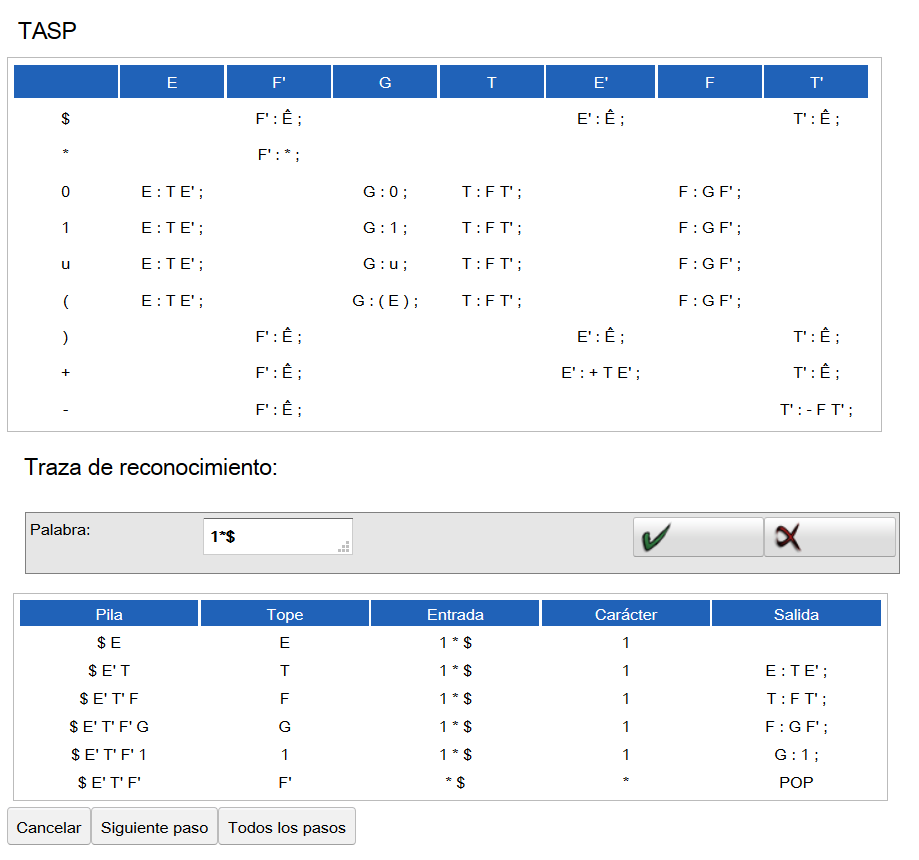
\includegraphics[width=1\textwidth]{reconocimiento-Tasp}
\caption{Vista del reconocimiento con TASP. Se aprecia la zona donde introducir la palabra y los botones.}
\label{fig:6.9}
\end{figure}

Volviendo al menú podemos apreciar que en las opciones aparece el nombre con el que se ha registrado el usuario. Si pulsamos en ello podremos ver como se despliega la opción para cerrar la sesión \ref{fig:6.10}. Al cerrar sesión se volverá a la vista de <<login>> y deberemos acceder de nuevo escribiendo el correo y la contraseña.

\begin{figure}[h]
\centering
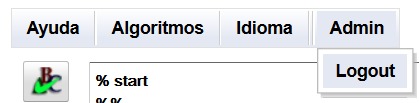
\includegraphics[width=0.40\textwidth]{menu-usuario}
\caption{Menú con el nombre del usuario. El desplegable muestra el cierre de la sesión.}
\label{fig:6.10}
\end{figure}

Siguiendo con el menú, la opción del idioma permite cambiar los textos de la aplicación, al idioma elegido \ref{fig:6.11}. Como la vista se va a reiniciar y la gramática desaparecerá, es necesario mostrar un mensaje que solicita confirmación adicional. Si pulsamos en <<si>> se llevará a cabo el reinicio, y como ya mantenemos una sesión activa, no sera necesario volver a iniciar sesión. Su pulsamos <<no>> el popup desaparecerá.

\begin{figure}[h]
\centering
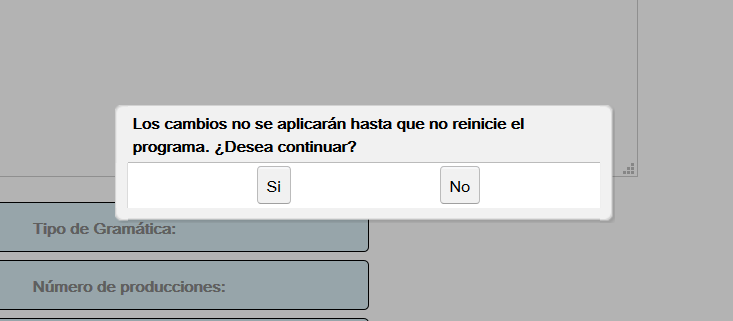
\includegraphics[width=0.40\textwidth]{opcion-idioma}
\caption{Mensaje de confirmación para cambiar el idioma.}
\label{fig:6.11}
\end{figure}




\bibliographystyle{plain}
\bibliography{bibliografiaAnexos}

\end{document}
